\section{Experimental methods and design choices}
\label{app:methods}

\subsection{Data generation}
We generate anisotropic Gaussian-mixture data:
\begin{itemize}\itemsep1pt
\item Cluster centers $\{m_c\}_{c=1}^{k}$ are drawn iid uniformly on a sphere
      of radius $s$ inside the first $\dint$ coordinates of $\mathbb{R}^{\dlat}$;
      the remaining $\dlat - \dint$ ``null-space'' coordinates of every
      center are exactly zero.
\item For each training point $\mu$, a cluster index $c(\mu)$ is drawn
      uniformly, then $x^{\mu} = m_{c(\mu)} + Q\,\xi^{\mu}$ where $\xi$
      has independent components: variance $\sigsig^2 = 1$ along the
      $\dint$ signal dimensions and variance $\signoise^2$ along the
      $\dlat - \dint$ null-space dimensions. $Q$ is a fixed orthogonal
      basis whose first $\dint$ columns span the signal subspace.
\item Default values: $k = 10$, $\dint = 5$, $s = 3$,
      $\nsamp = 500$ training points, $2048$ held-out test points,
      $\sigsig = 1$, $\signoise \in \{0.01, 0.5\}$.
\end{itemize}

\subsection{Diffusion process}
We use the variance-preserving Ornstein-Uhlenbeck process with
$t \in [t_{\min}, t_{\max}] = [0.01, 3.0]$. Score targets are computed
analytically from the closed-form Gaussian-mixture density at noise level $t$;
this avoids the standard score-matching MSE loss noise floor and gives a
clean ``score error'' metric independent of training-set fluctuations.

\subsection{Models}
\paragraph{MLP.} 3-layer ReLU MLP with sinusoidal time embedding ($32$
frequency bands), input width $\dlat + 64$, output width $\dlat$.
Hidden width $h = 256$ held fixed across the $\dlat$ sweep. Adam with
learning rate $10^{-4}$, batch size $256$, $T = 3\times 10^5$ training
steps (extended to $5\times 10^6$ for the body timescale-scatter
figure), evaluation every $5{,}000$ steps with $5{,}000$ generated
samples.

\paragraph{RFNN.} Two-layer RFNN with $\tanh$ activation; first layer
$W \in \mathbb{R}^{\pwidth \times \dlat}$ is fixed at random Gaussian
initialization, the second-layer readout $A$ is trained. $\pwidth = 64\,\dlat$
to keep the rank-null bulk visible at every $\dlat$. Same optimizer, batch,
and evaluation cadence as the MLP.

\subsection{Evaluation metrics}
\begin{itemize}\itemsep1pt
\item \textbf{Score error}: integrated mean-squared error of the learned
      score against the analytic Gaussian-mixture score, averaged over
      $5{,}000$ test points.
\item \textbf{Memorization fraction}: fraction of generated samples whose
      nearest training-set neighbor is closer than one third of that
      neighbor's own nearest training-set
      neighbor~\citep{somepalli2023diffusion}.
\item \textbf{$\taugen$}: first step at which test loss is within $5\%$ of
      its per-run minimum.
\item \textbf{$\taumem$}: first step at which the memorization fraction
      exceeds $1\%$. Censored to ``$>$300k'' if not crossed within budget.
\end{itemize}

\paragraph{Why these definitions.}
We use the test-loss-plateau criterion for $\taugen$ rather than an FID-
or MMD-based criterion because (i) it is well-defined on both the MLP
and the RFNN, the latter trained at fixed $t$ with no usable generation
process, (ii) the analytic Gaussian-mixture score gives noise-floor-free
target values, removing the need for finite-sample FID estimates that
fluctuate with the number of generated samples, and (iii) the test-loss
plateau aligns directly with the moment when the population score has
been internalised. We use the \citet{somepalli2023diffusion}-style
memorization fraction for $\taumem$ on the MLP because it is the same
threshold \citet{bonnaire2025} use, allowing direct comparison with the
isotropic baseline. For the fixed-$t$ RFNN, no generation is available;
we substitute the gen-gap proxy ($\text{test loss} - \text{train loss}
> 0.02$), which monotonically tracks the canonical $\taumem$ on the MLP
and calibrates the two-track comparison.

\subsection{Per-experiment configurations}
\label{app:exp-configs}

Both sweeps (Section~\ref{sec:design}, ``Two complementary sweeps'')
run on the synthetic Gaussian-mixture data described above. Shared
constants across every run: $\nsamp = 500$ training points, $2{,}048$
held-out test points, $k = 10$ cluster centers, $s = 3$, $\sigsig = 1$,
OU diffusion at $t \in [0.01, 3.0]$, seed $42$ for both data and the
random first layer $W$. Tables~\ref{tab:exp-configs}
and~\ref{tab:exp-hparams} list the sweeps and training
hyperparameters.

\begin{table}[!t]
\centering\small
\setlength{\tabcolsep}{4pt}
\caption{\textbf{Sweep configurations.} Both $\signoise$ values used
unless noted.}
\label{tab:exp-configs}
\begin{tabular}{@{}lllll@{}}
\toprule
Model & Vary & Range & Fixed & Width \\
\midrule
MLP                       & $\dlat$ & $\{5, 8, 10, 15, 20, 30, 40\}$ & $\dint = 5$ & $h = 256$ \\
RFNN                      & $\dlat$ & $\{5, 8, 10, 15, 20, 30, 40\}$ & $\dint = 5$ & $\pwidth = 64\,\dlat$ \\
RFNN (ext., $\signoise{=}0.5$) & $\dlat$ & $\{60, 80, 100, 150, 200\}$ & $\dint = 5$ & $\pwidth = 64\,\dlat$ \\
MLP                       & $\dint$ & $\{2, 5, 8, 12, 16, 20\}$ & $\dlat = 20$ & $h = 256$ \\
RFNN                      & $\dint$ & $\{2, 5, 8, 12, 16, 20\}$ & $\dlat = 20$ & $\pwidth = 1280$ \\
\bottomrule
\end{tabular}
\end{table}

\begin{table}[!t]
\centering\small
\setlength{\tabcolsep}{6pt}
\caption{\textbf{Training hyperparameters.}}
\label{tab:exp-hparams}
\begin{tabular}{@{}lll@{}}
\toprule
 & MLP & RFNN \\
\midrule
Optimizer & Adam & full-batch GD \\
Learning rate & $10^{-4}$ & closed-form \\
Batch size & $256$ & full ($\nsamp = 500$) \\
Total steps $T$ & $3 \times 10^5$ & $3 \times 10^5$ \\
Eval interval & $5{,}000$ & $5{,}000$ \\
Diffusion time & $t \sim \mathrm{Unif}[0.01, 3.0]$ & fixed $t = 0.01$ \\
Time embedding & sinusoidal, $32$ frequencies & n/a\\
Activation & ReLU & $\tanh$ \\
$\Umat$ Monte Carlo & n/a& $50$ noise samples per training point \\
\bottomrule
\end{tabular}
\end{table}

\subsection{Empirical bulk sizes}
\label{app:bulk-sizes}
Table~\ref{tab:bulk-sizes} reports the per-panel sizes of the four
detected bulks in Figure~\ref{fig:bulk-sizes-distances}, ordered
left-to-right by increasing eigenvalue (B1: rank-null tail; B4:
signal block). $\signoise = 0.01$, $\dint = 5$, $\nsamp = 500$,
$\pwidth = 64\,\dlat$.

\begin{table}[!t]
\centering\small
\setlength{\tabcolsep}{6pt}
\caption{\textbf{Empirical bulk sizes per $\dlat$.} B4 collapses to
$\dint = 5$ as predicted; B3 grows linearly with $\dlat - \dint$
(the noise-dim buffer); B1 absorbs the rank-null tail.}
\label{tab:bulk-sizes}
\begin{tabular}{@{}rrrrr@{}}
\toprule
$\dlat$ & B1 & B2 & B3 & B4 \\
\midrule
5  & 150  & 138 & 27 & 5 \\
8  & 344  & 133 & 30 & 5 \\
10 & 295  & 305 & 35 & 5 \\
15 & 699  & 216 & 40 & 5 \\
20 & 916  & 311 & 48 & 5 \\
30 & 1397 & 458 & 60 & 5 \\
40 & 1907 & 578 & 70 & 5 \\
\bottomrule
\end{tabular}
\end{table}

\subsection{Known pitfalls}
The $\tanh$ activation in the RFNN saturates whenever the data scale
divided by $\sqrt{\dlat}$ exceeds approximately $2$, collapsing all
eigenvalues into a degenerate single bulk. Configurations were chosen to
keep the operating point well inside the linear regime; see
Appendix~\ref{app:saturation}.

% ===== MLP block (sec 3 in the body) ===========================

\section{$\dlat$ sweep (synthetic data)}
\label{app:mlp-dlat-sweep}

The body reports the updated five-seed $\dlat$ sweep at fixed
$\dint=5$ (Figs.~\ref{fig:synthetic-mlp-final-mem}--
\ref{fig:synthetic-mlp-score-error}). This appendix preserves the
older synthetic diagnostic views: timescales, late gen-gap, and
score-error curves for both the $\dlat$ and $\dint$ sweeps.

\begin{figure}[!t]
  \centering
  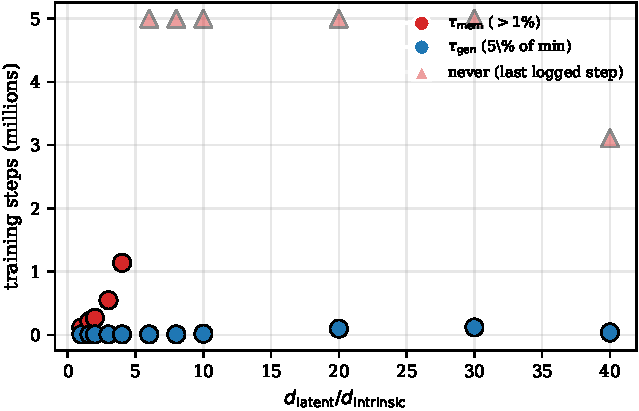
\includegraphics[width=0.85\linewidth]{figures/mlp_timescales_scatter.pdf}
  \caption{\textbf{$\dlat$ sweep: timescales versus $\dlat / \dint$
    at $\signoise = 0.5$.} 5M-step MLP. Triangles mark runs that do
    not reach $1\%$ memorization within budget.}
  \label{fig:mlp-dlat-timescales}
\end{figure}

\begin{figure}[!t]
  \centering
  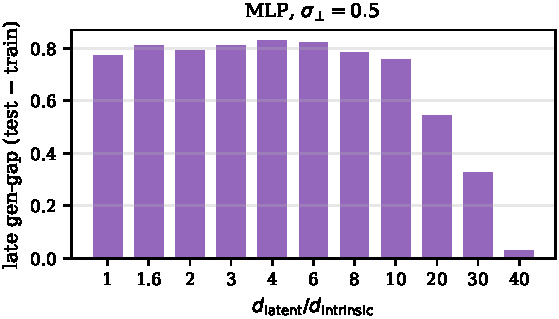
\includegraphics[width=0.7\linewidth]{figures/mlp_gen_gap_sn05.pdf}
  \caption{\textbf{$\dlat$ sweep: late generalization gap versus
    $\dlat / \dint$ at $\signoise = 0.5$.}}
  \label{fig:mlp-dlat-gen-gap}
\end{figure}

\begin{figure}[!t]
  \centering
  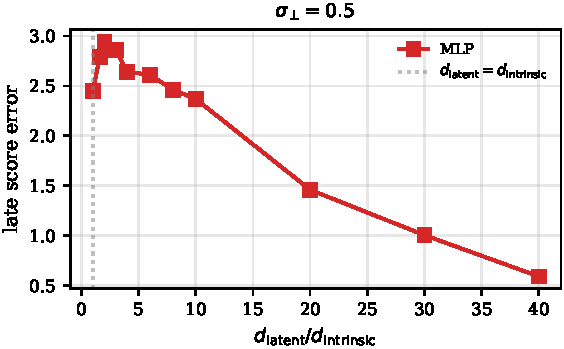
\includegraphics[width=0.7\linewidth]{figures/late_score_error_sn05.pdf}
  \caption{\textbf{$\dlat$ sweep: late score error versus
    $\dlat / \dint$ at $\signoise = 0.5$. Compare with the updated
    normalized score-error trajectories in
    Fig.~\ref{fig:synthetic-mlp-score-error}.}}
  \label{fig:mlp-dlat-late-score}
\end{figure}

\begin{figure}[!t]
  \centering
  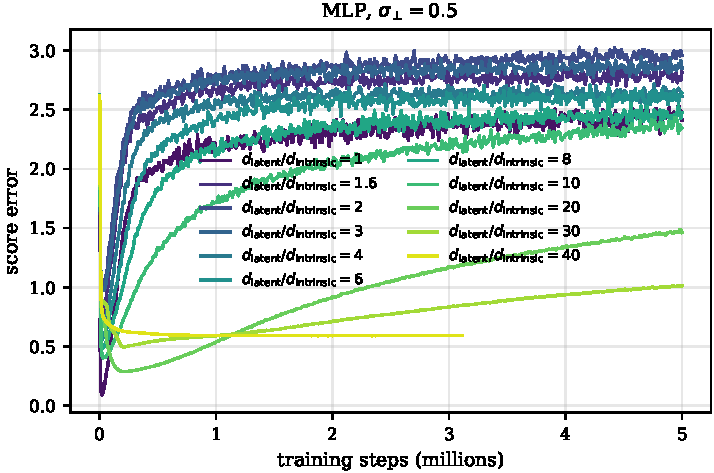
\includegraphics[width=0.85\linewidth]{figures/mlp_score_error_curves_sn05.pdf}
  \caption{\textbf{$\dlat$ sweep: score error over training at
    $\signoise = 0.5$.} Per-step trajectories underlying the
    aggregate in Fig.~\ref{fig:mlp-dlat-late-score}, one curve per
    $\dlat$ (viridis colormap, low to high). Compare to
    Fig.~\ref{fig:mlp-dint-score-curves} (the $\dint$-sweep
    counterpart).}
  \label{fig:mlp-dlat-score-curves}
\end{figure}

\begin{figure}[!t]
  \centering
  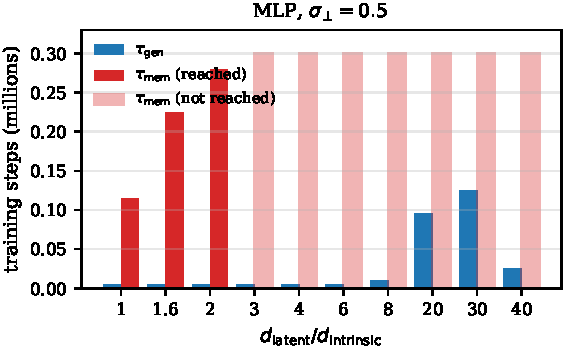
\includegraphics[width=0.7\linewidth]{figures/mlp_timescales_bar_sn05.pdf}
  \caption{\textbf{$\dlat$ sweep: 300k-step bar-chart timescales at
    $\signoise = 0.5$.} The 300k-step bar-chart view of paired
    $\taugen$ (blue) and $\taumem$ (red), with hatched bars
    indicating $\taumem$ not reached within budget. The 5M-step
    extended-budget version is Fig.~\ref{fig:mlp-dlat-timescales}
    above.}
  \label{fig:mlp-dlat-timescales-bar}
\end{figure}

\section{$\dlat$ sweep at $\signoise = 0.01$}
\label{app:mlp-sn001}

The $\signoise = 0.01$ counterparts of the $\dlat$ sweep figures
in Appendix~\ref{app:mlp-dlat-sweep}. The non-monotonic score-error
peak discussed in Sec.~\ref{sec:discussion} is visible in
Fig.~\ref{fig:mlp-dlat-late-score-sn001}.

\begin{figure}[!t]
  \centering
  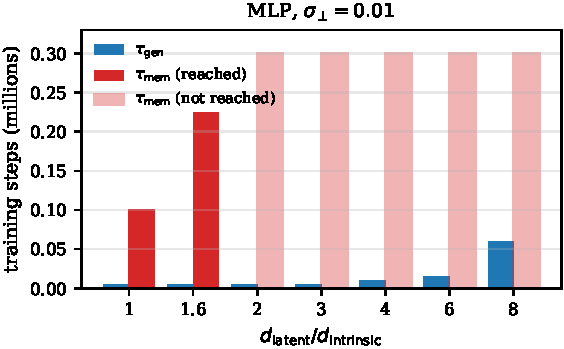
\includegraphics[width=0.7\linewidth]{figures/mlp_timescales_bar_sn001.pdf}
  \caption{\textbf{$\signoise = 0.01$ counterpart of
    Fig.~\ref{fig:mlp-dlat-timescales-bar}.}}
  \label{fig:mlp-dlat-timescales-sn001}
\end{figure}

\begin{figure}[!t]
  \centering
  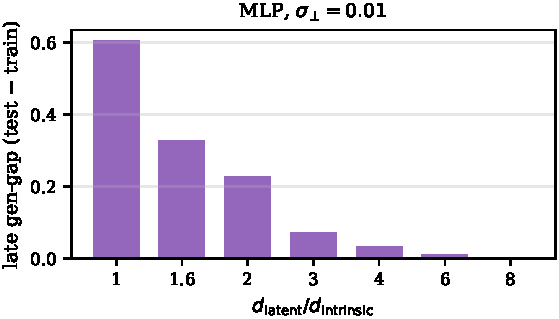
\includegraphics[width=0.7\linewidth]{figures/mlp_gen_gap_sn001.pdf}
  \caption{\textbf{$\signoise = 0.01$ counterpart of
    Fig.~\ref{fig:mlp-dlat-gen-gap}.}}
  \label{fig:mlp-dlat-gen-gap-sn001}
\end{figure}

\begin{figure}[!t]
  \centering
  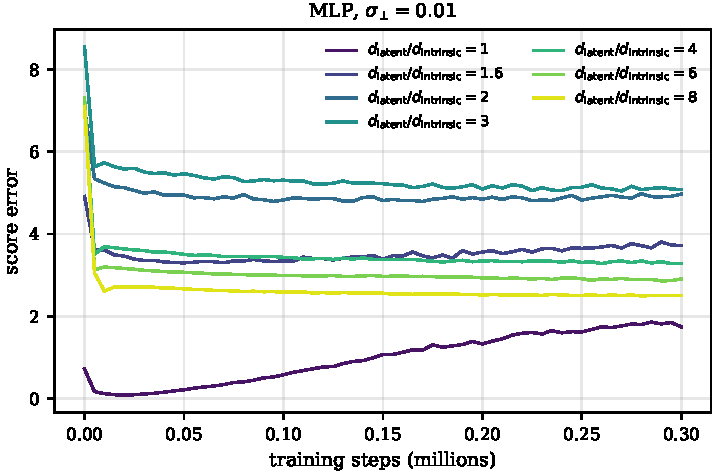
\includegraphics[width=0.7\linewidth]{figures/mlp_score_error_curves_sn001.pdf}
  \caption{\textbf{$\signoise = 0.01$ counterpart of
    Fig.~\ref{fig:mlp-dlat-score-curves}.}}
  \label{fig:mlp-dlat-score-curves-sn001}
\end{figure}

\begin{figure}[!t]
  \centering
  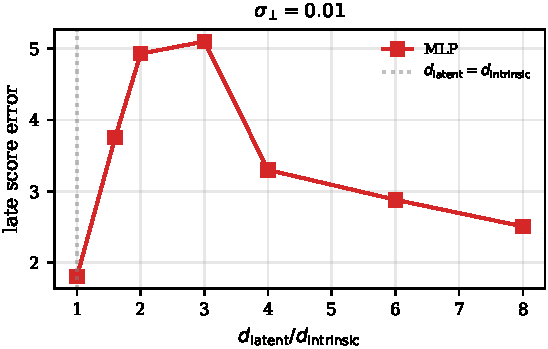
\includegraphics[width=0.7\linewidth]{figures/late_score_error_sn001.pdf}
  \caption{\textbf{$\signoise = 0.01$ counterpart of
    Fig.~\ref{fig:mlp-dlat-late-score}.} The non-monotonic peak
    discussed in Sec.~\ref{sec:discussion} is visible here.}
  \label{fig:mlp-dlat-late-score-sn001}
\end{figure}

\section{$\dint$ sweep additional figures}
\label{app:mlp-dint}

This section collects additional $\dint$-sweep diagnostics at fixed
$\dlat=20$, complementary to the updated $\dlat$-sweep MLP figures
in the body.

\begin{figure}[!t]
  \centering
  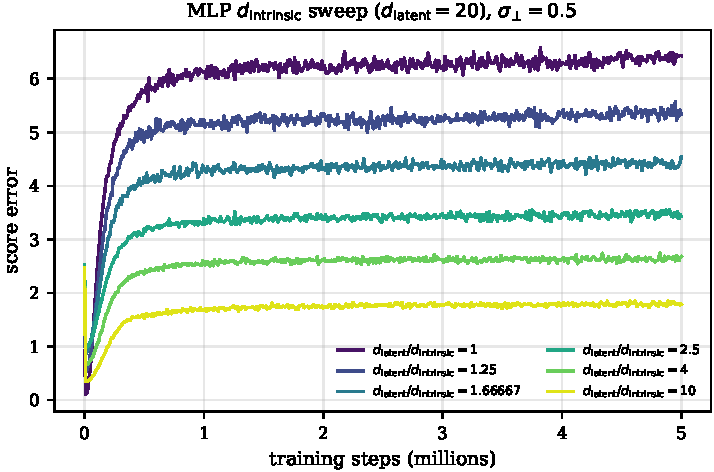
\includegraphics[width=0.85\linewidth]{figures/mlp_dint_score_curves_sn05.pdf}
  \caption{\textbf{$\dint$ sweep: score error over training at
    $\signoise = 0.5$.} One curve per $\dlat / \dint$ ratio
    (viridis colormap). Per-step trajectories underlying the
    body's $\dint$-sweep aggregates.}
  \label{fig:mlp-dint-score-curves}
\end{figure}

\begin{figure}[!t]
  \centering
  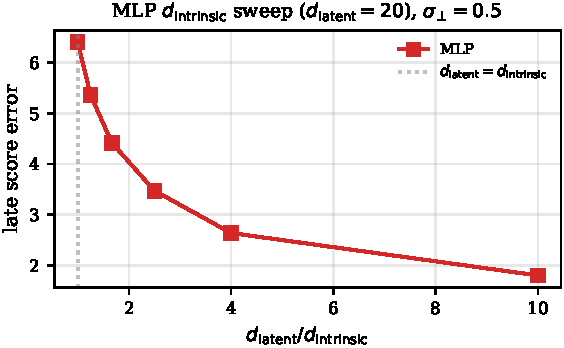
\includegraphics[width=0.7\linewidth]{figures/mlp_dint_late_score_sn05.pdf}
  \caption{\textbf{$\dint$ sweep: late score error versus
    $\dlat / \dint$ at $\signoise = 0.5$.} $\dint$-sweep counterpart
    of the wider-range $\dlat$ sweep.}
  \label{fig:mlp-dint-late-score}
\end{figure}

\section{$\dint$ sweep at $\signoise = 0.01$}
\label{app:mlp-dint-sn001}

The $\signoise = 0.01$ counterparts of the body's $\dint$ sweep at
fixed $\dlat = 20$. These runs are at 300k training steps (the 5M
extension was only run at $\signoise = 0.5$).

\begin{figure}[!t]
  \centering
  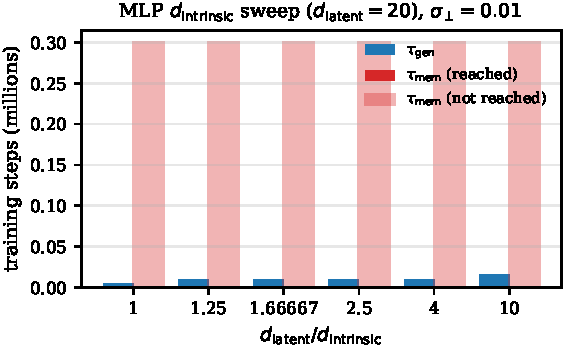
\includegraphics[width=0.7\linewidth]{figures/mlp_dint_timescales_sn001.pdf}
  \caption{\textbf{$\signoise = 0.01$ $\dint$-sweep timescales.}}
  \label{fig:mlp-dint-timescales-sn001}
\end{figure}

\begin{figure}[!t]
  \centering
  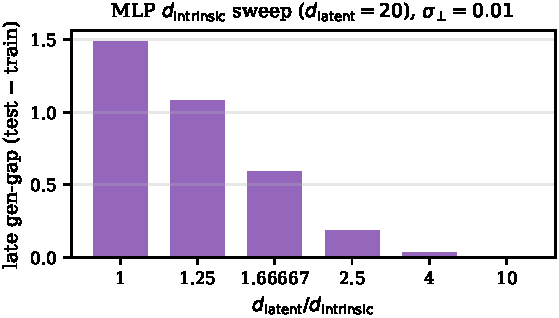
\includegraphics[width=0.7\linewidth]{figures/mlp_dint_gen_gap_sn001.pdf}
  \caption{\textbf{$\signoise = 0.01$ $\dint$-sweep gen-gap.}}
  \label{fig:mlp-dint-gen-gap-sn001}
\end{figure}

\begin{figure}[!t]
  \centering
  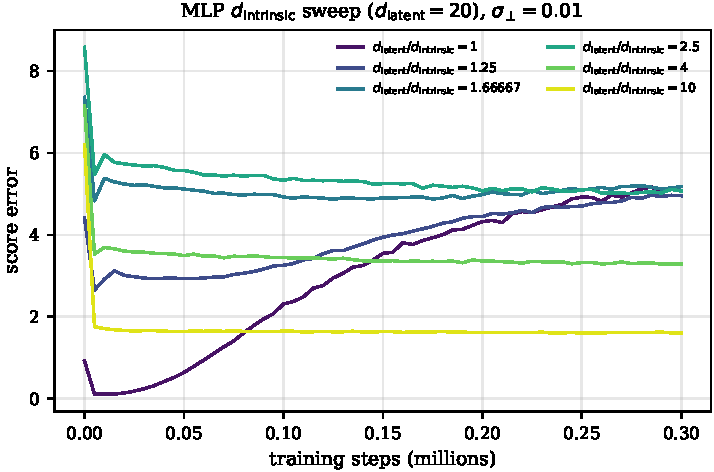
\includegraphics[width=0.85\linewidth]{figures/mlp_dint_score_curves_sn001.pdf}
  \caption{\textbf{$\signoise = 0.01$ counterpart of
    Fig.~\ref{fig:mlp-dint-score-curves}.}}
  \label{fig:mlp-dint-score-curves-sn001}
\end{figure}

\begin{figure}[!t]
  \centering
  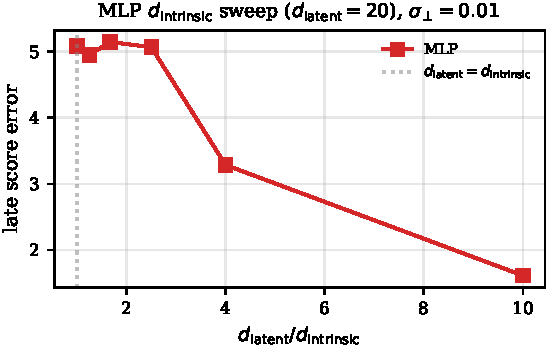
\includegraphics[width=0.7\linewidth]{figures/mlp_dint_late_score_sn001.pdf}
  \caption{\textbf{$\signoise = 0.01$ $\dint$-sweep late score error.}}
  \label{fig:mlp-dint-late-score-sn001}
\end{figure}

\section{Real-data experiments}
\label{app:real-data}

\subsection{Setup}
We test the buffer mechanism on CelebA and CIFAR-10, with the
latent space learned by a VAE. For each dataset and latent
dimension, the VAE is trained on the full available training split.
The diffusion model is then trained on a diverse 1k-image subset of
the encoded training set. The score model is the fixed-width MLP
from Sec.~\ref{sec:mlp}: 3-layer ReLU network, sinusoidal time
embedding, five seeds, 5M training steps, FID evaluated every
100k steps, and pixel-space memorization evaluated by the
Bonnaire/Somepalli nearest-neighbor ratio test.

\paragraph{Latent sweeps.}
CelebA uses $\dlat \in \{10,20,\ldots,100,120,140,160,180,200\}$.
CIFAR-10 uses
$\dlat \in \{20,40,\ldots,200,220,240,260\}$. The high-dimensional
CIFAR-10 runs exclude exploratory gradient-clipped seeds because
clipping substantially suppressed memorization; replacement seeds
use the same optimizer and learning rate as the rest of the sweep.

\subsection{VAE diagnostics}
The VAE itself creates a measurable confound: if the bottleneck is
too small, encode--decode reconstructions are too blurred to count
as pixel-space memorization. We therefore report VAE validation
metrics and reconstruction memorization separately from the
diffusion model.

\begin{figure}[!t]
  \centering
  \begin{subfigure}{0.49\linewidth}
    \centering
    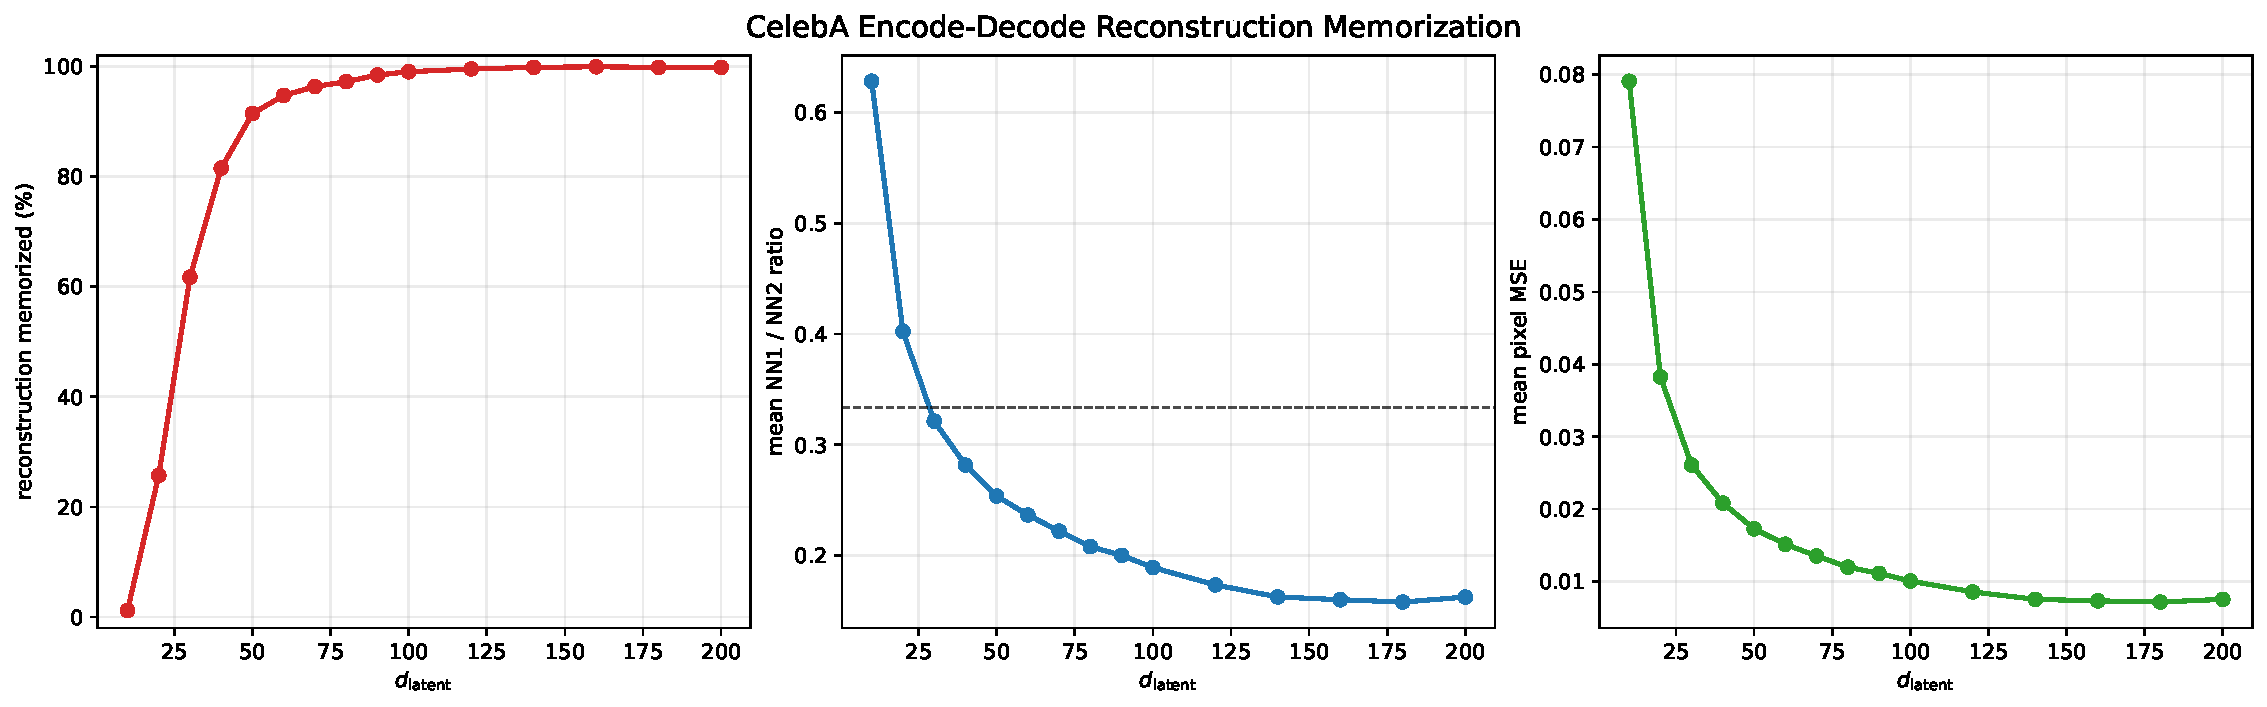
\includegraphics[width=\linewidth]{figures/vae_diagnostics/celeba_reconstruction_mem_vs_d.pdf}
    \caption{CelebA.}
  \end{subfigure}\hfill
  \begin{subfigure}{0.49\linewidth}
    \centering
    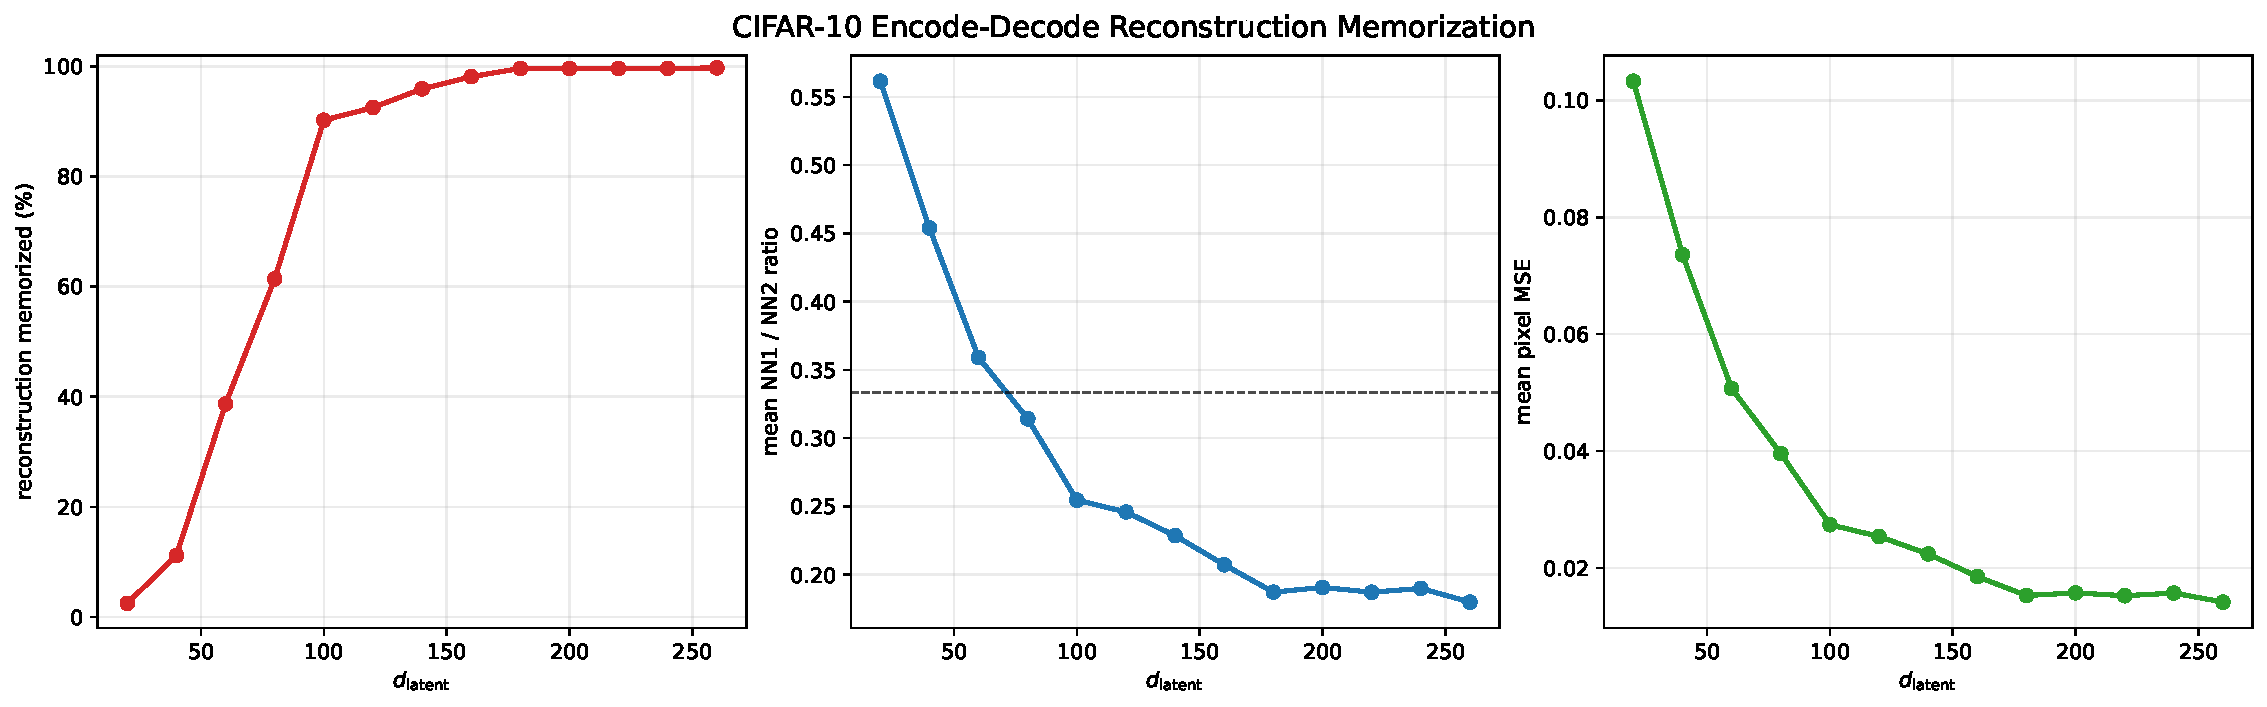
\includegraphics[width=\linewidth]{figures/vae_diagnostics/cifar10_reconstruction_mem_vs_d.pdf}
    \caption{CIFAR-10.}
  \end{subfigure}
  \caption{\textbf{VAE encode--decode reconstruction memorization.}
    The same Bonnaire/Somepalli nearest-neighbor ratio test is
    applied to VAE reconstructions of the diverse 1k subset. Low
    $\dlat$ VAEs reconstruct too poorly to trigger the pixel-space
    memorization test; higher $\dlat$ reconstructions increasingly
    return to their original training examples.}
  \label{fig:vae-reconstruction-mem}
\end{figure}

\begin{figure}[!t]
  \centering
  \begin{subfigure}{0.49\linewidth}
    \centering
    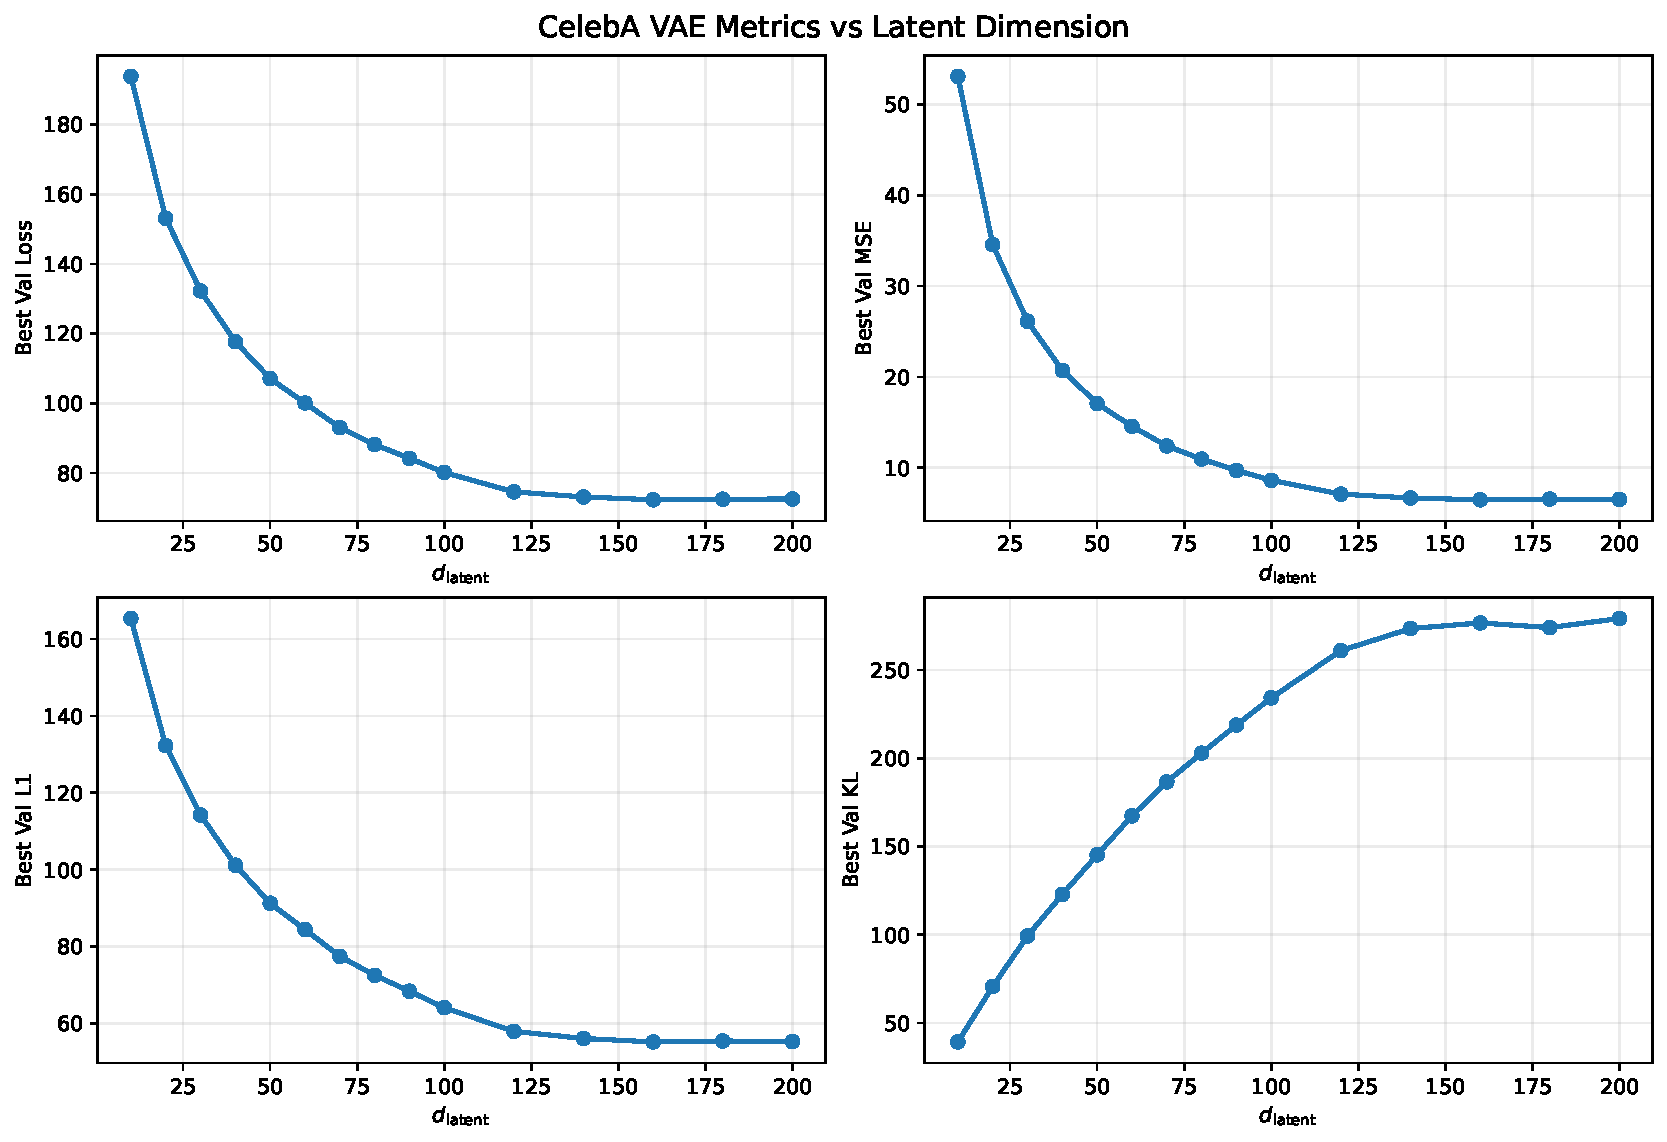
\includegraphics[width=\linewidth]{figures/vae_diagnostics/celeba_vae_metrics_vs_d.pdf}
    \caption{CelebA.}
  \end{subfigure}\hfill
  \begin{subfigure}{0.49\linewidth}
    \centering
    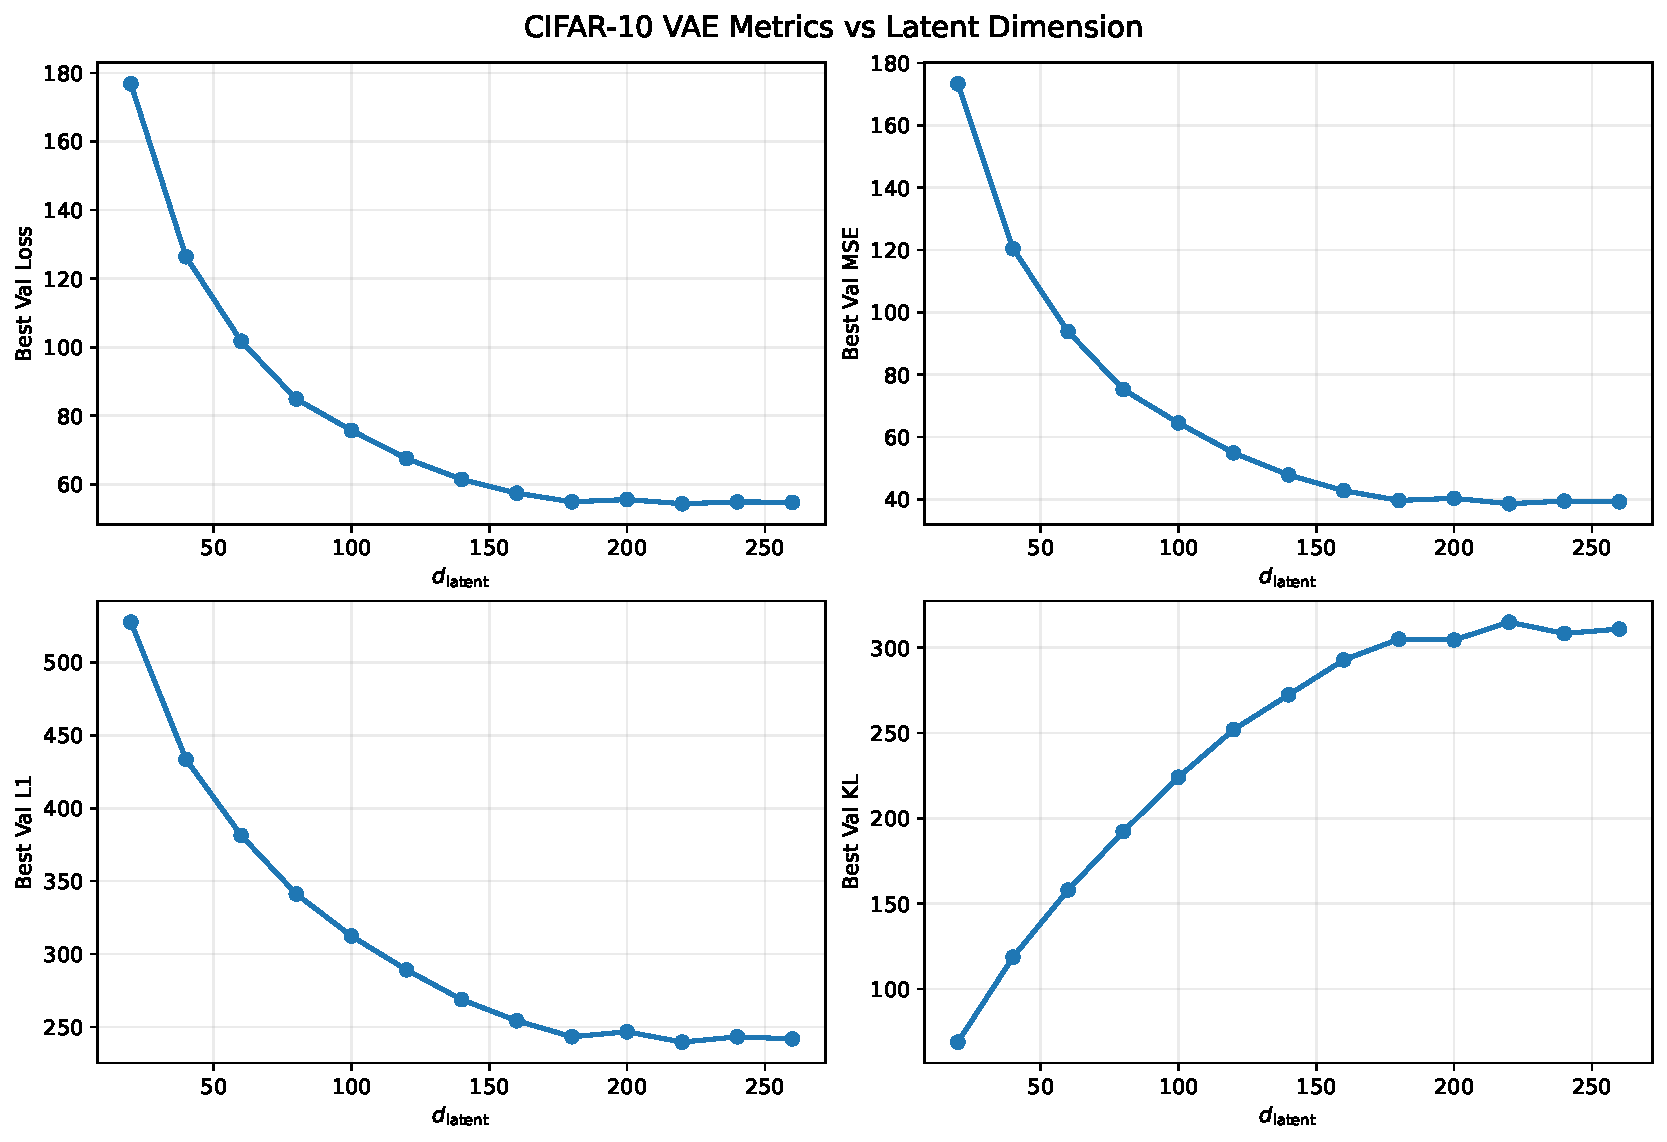
\includegraphics[width=\linewidth]{figures/vae_diagnostics/cifar10_vae_metrics_vs_d.pdf}
    \caption{CIFAR-10.}
  \end{subfigure}
  \caption{\textbf{VAE validation metrics.} Reconstruction loss,
    MSE, L1, and KL across the latent-dimension sweep. These curves
    explain the rising side of the real-data memorization plots:
    before the VAE is expressive enough, the diffusion model cannot
    reproduce training images sharply in pixel space.}
  \label{fig:vae-metrics}
\end{figure}

\subsection{Per-dimension diffusion trajectories}

\begin{figure}[!t]
  \centering
  \begin{subfigure}{0.49\linewidth}
    \centering
    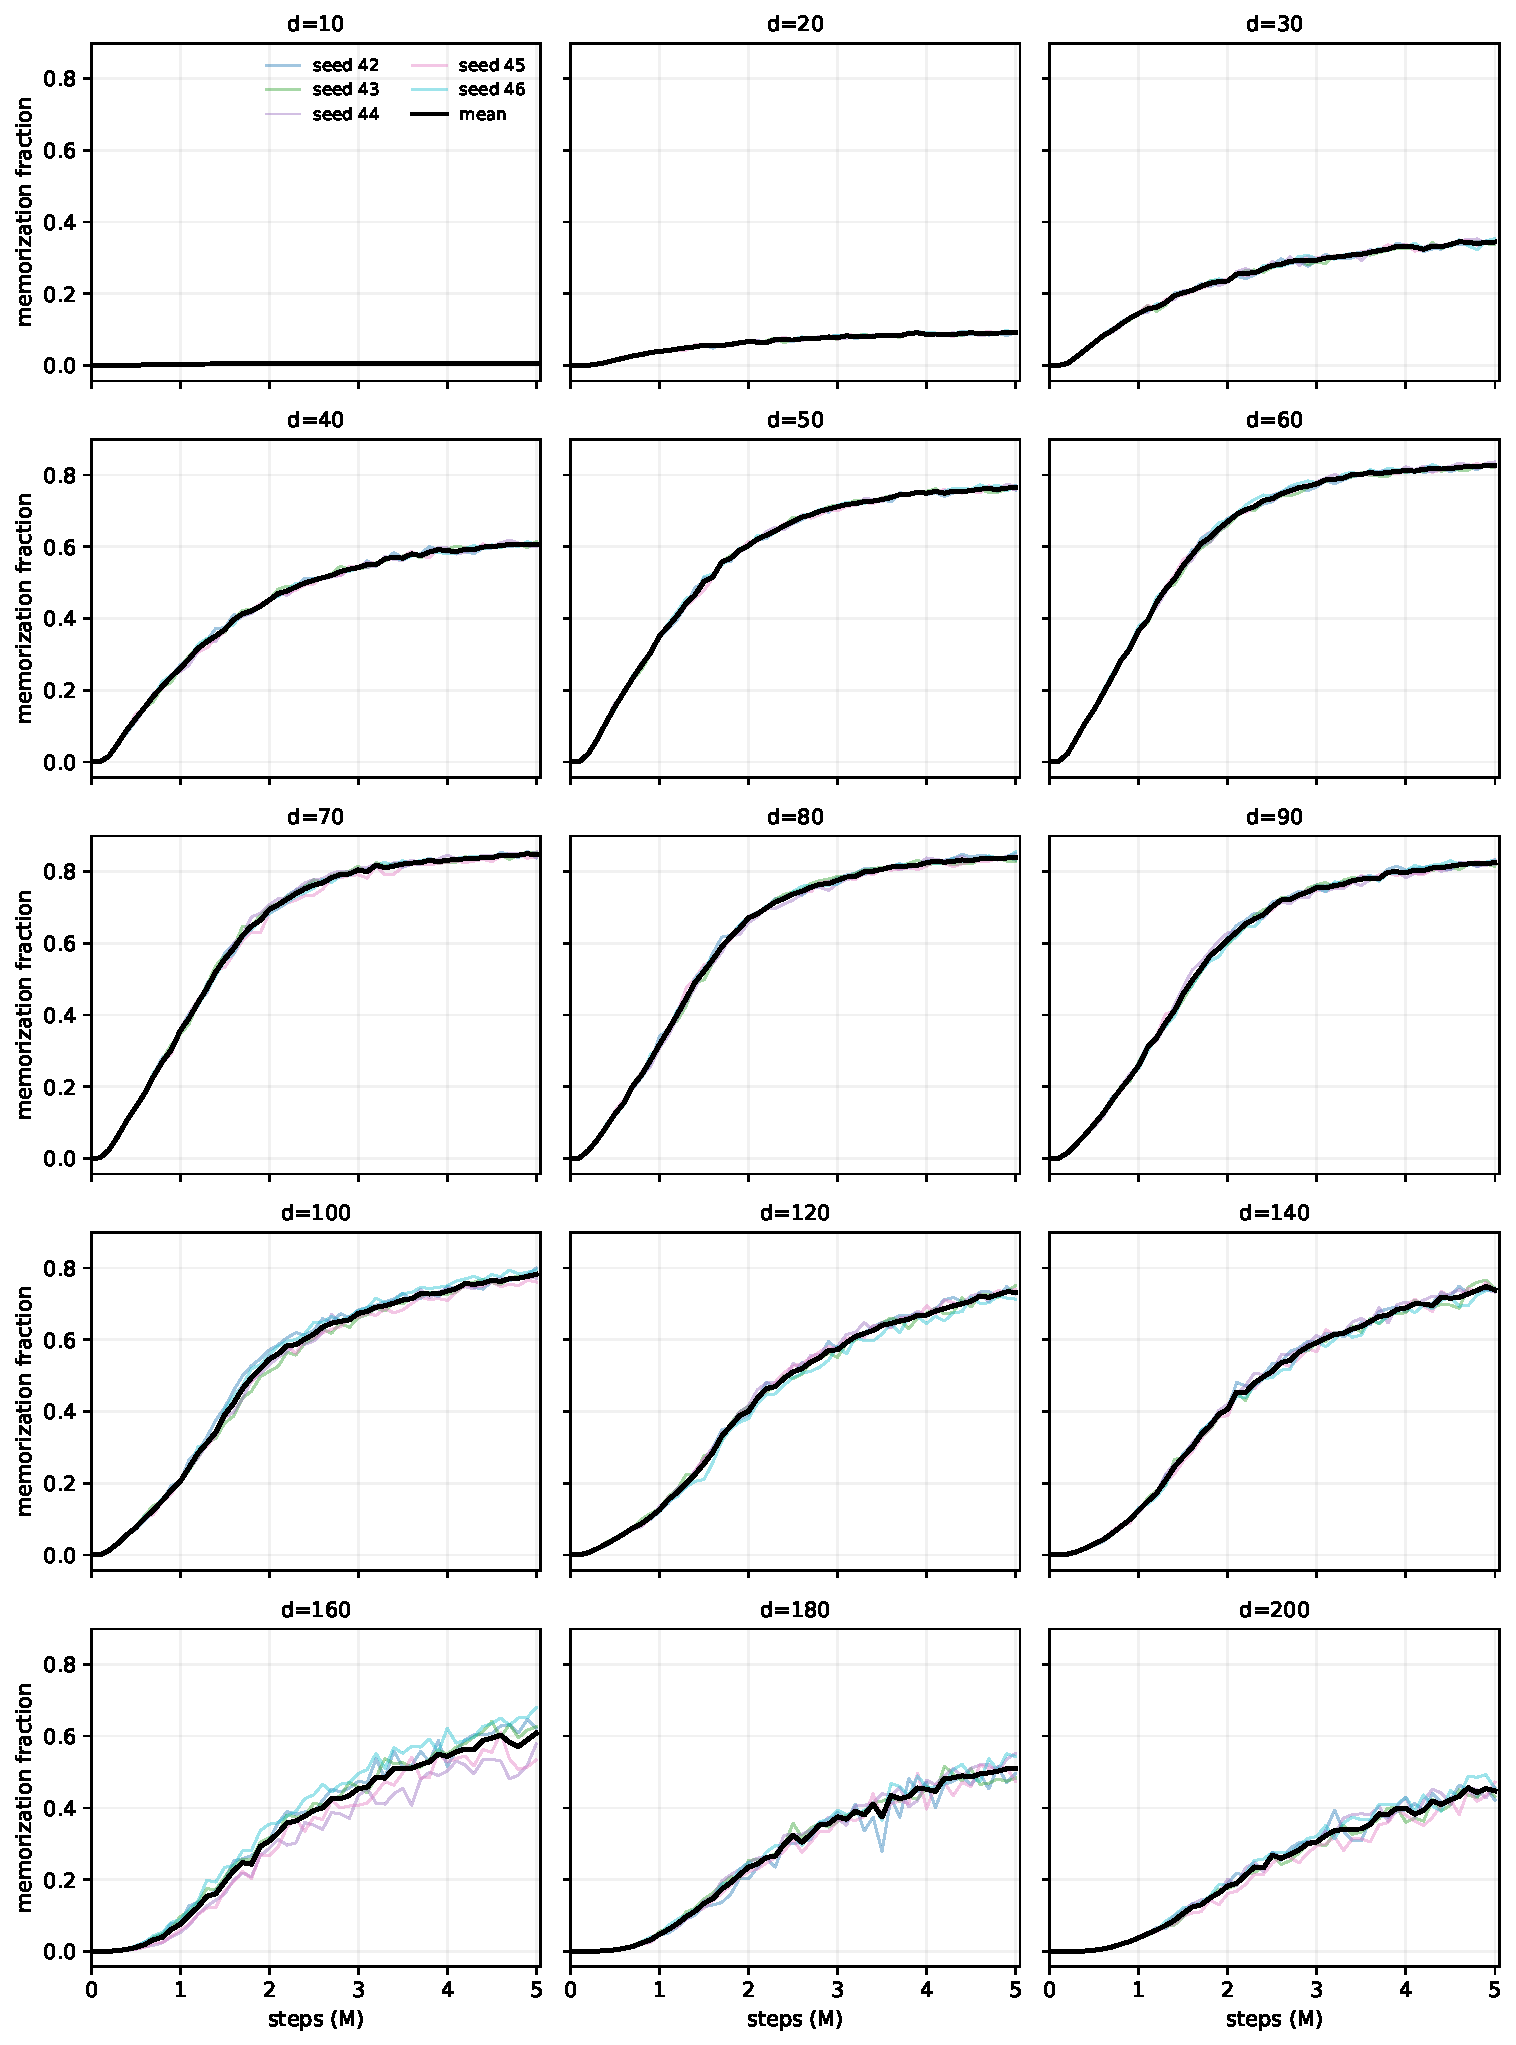
\includegraphics[width=\linewidth]{figures/celeba_individual_mem_by_d_over_steps.pdf}
    \caption{CelebA memorization.}
  \end{subfigure}\hfill
  \begin{subfigure}{0.49\linewidth}
    \centering
    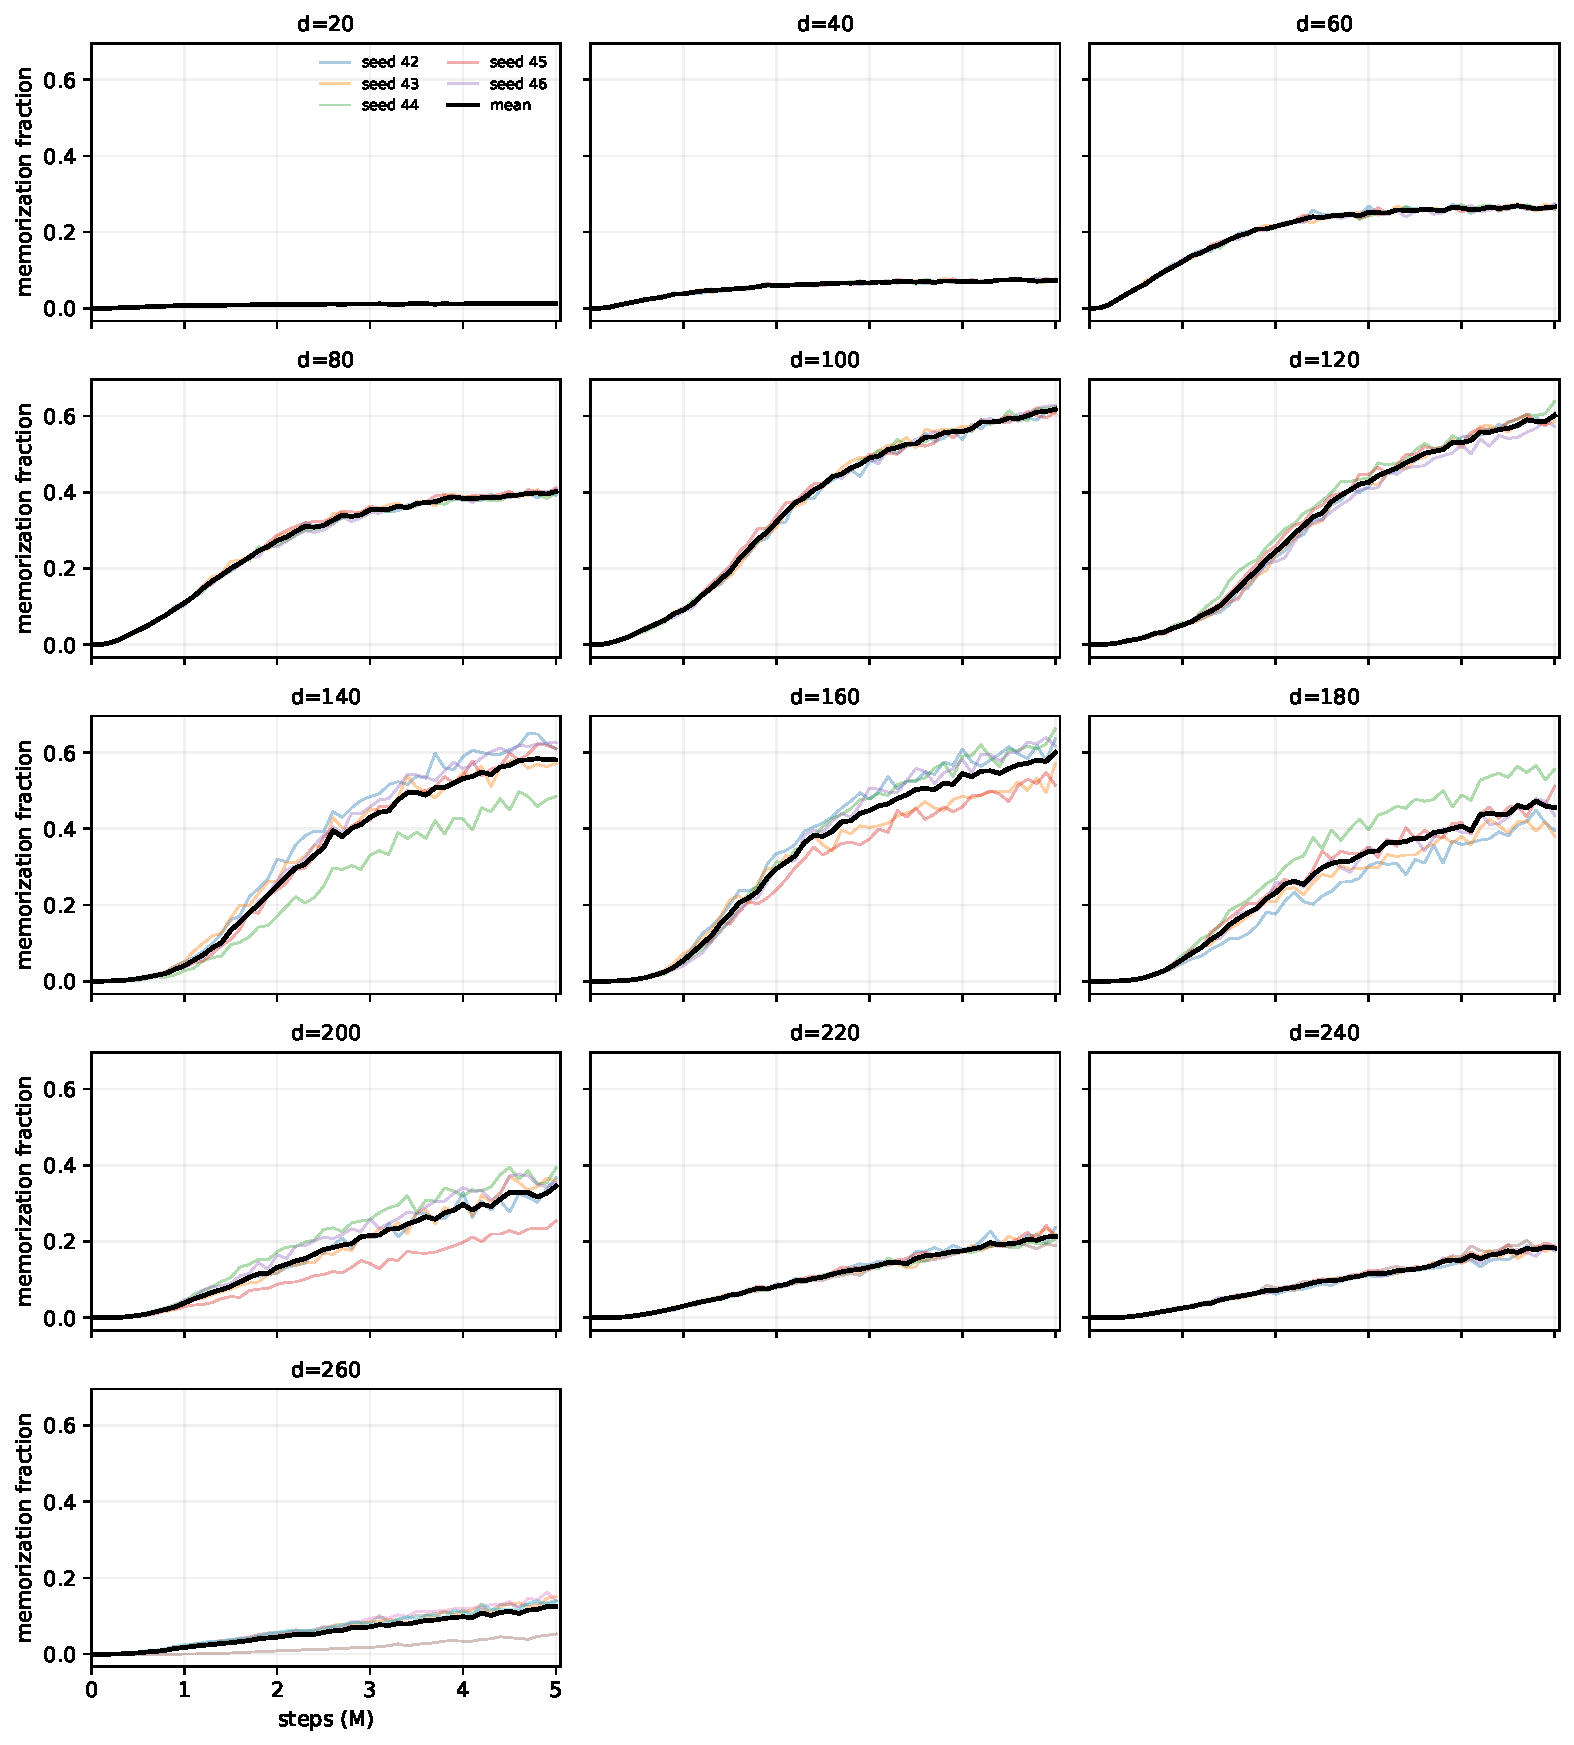
\includegraphics[width=\linewidth]{figures/cifar10_individual_mem_by_d_over_steps.pdf}
    \caption{CIFAR-10 memorization.}
  \end{subfigure}
  \caption{\textbf{Per-$\dlat$ memorization trajectories.} Each
    panel fixes one latent dimension and shows all five seeds plus
    their mean. The individual source PDFs are also included under
    \texttt{figures/real\_per\_d/}.}
  \label{fig:real-per-d-mem}
\end{figure}

\begin{figure}[!t]
  \centering
  \begin{subfigure}{0.49\linewidth}
    \centering
    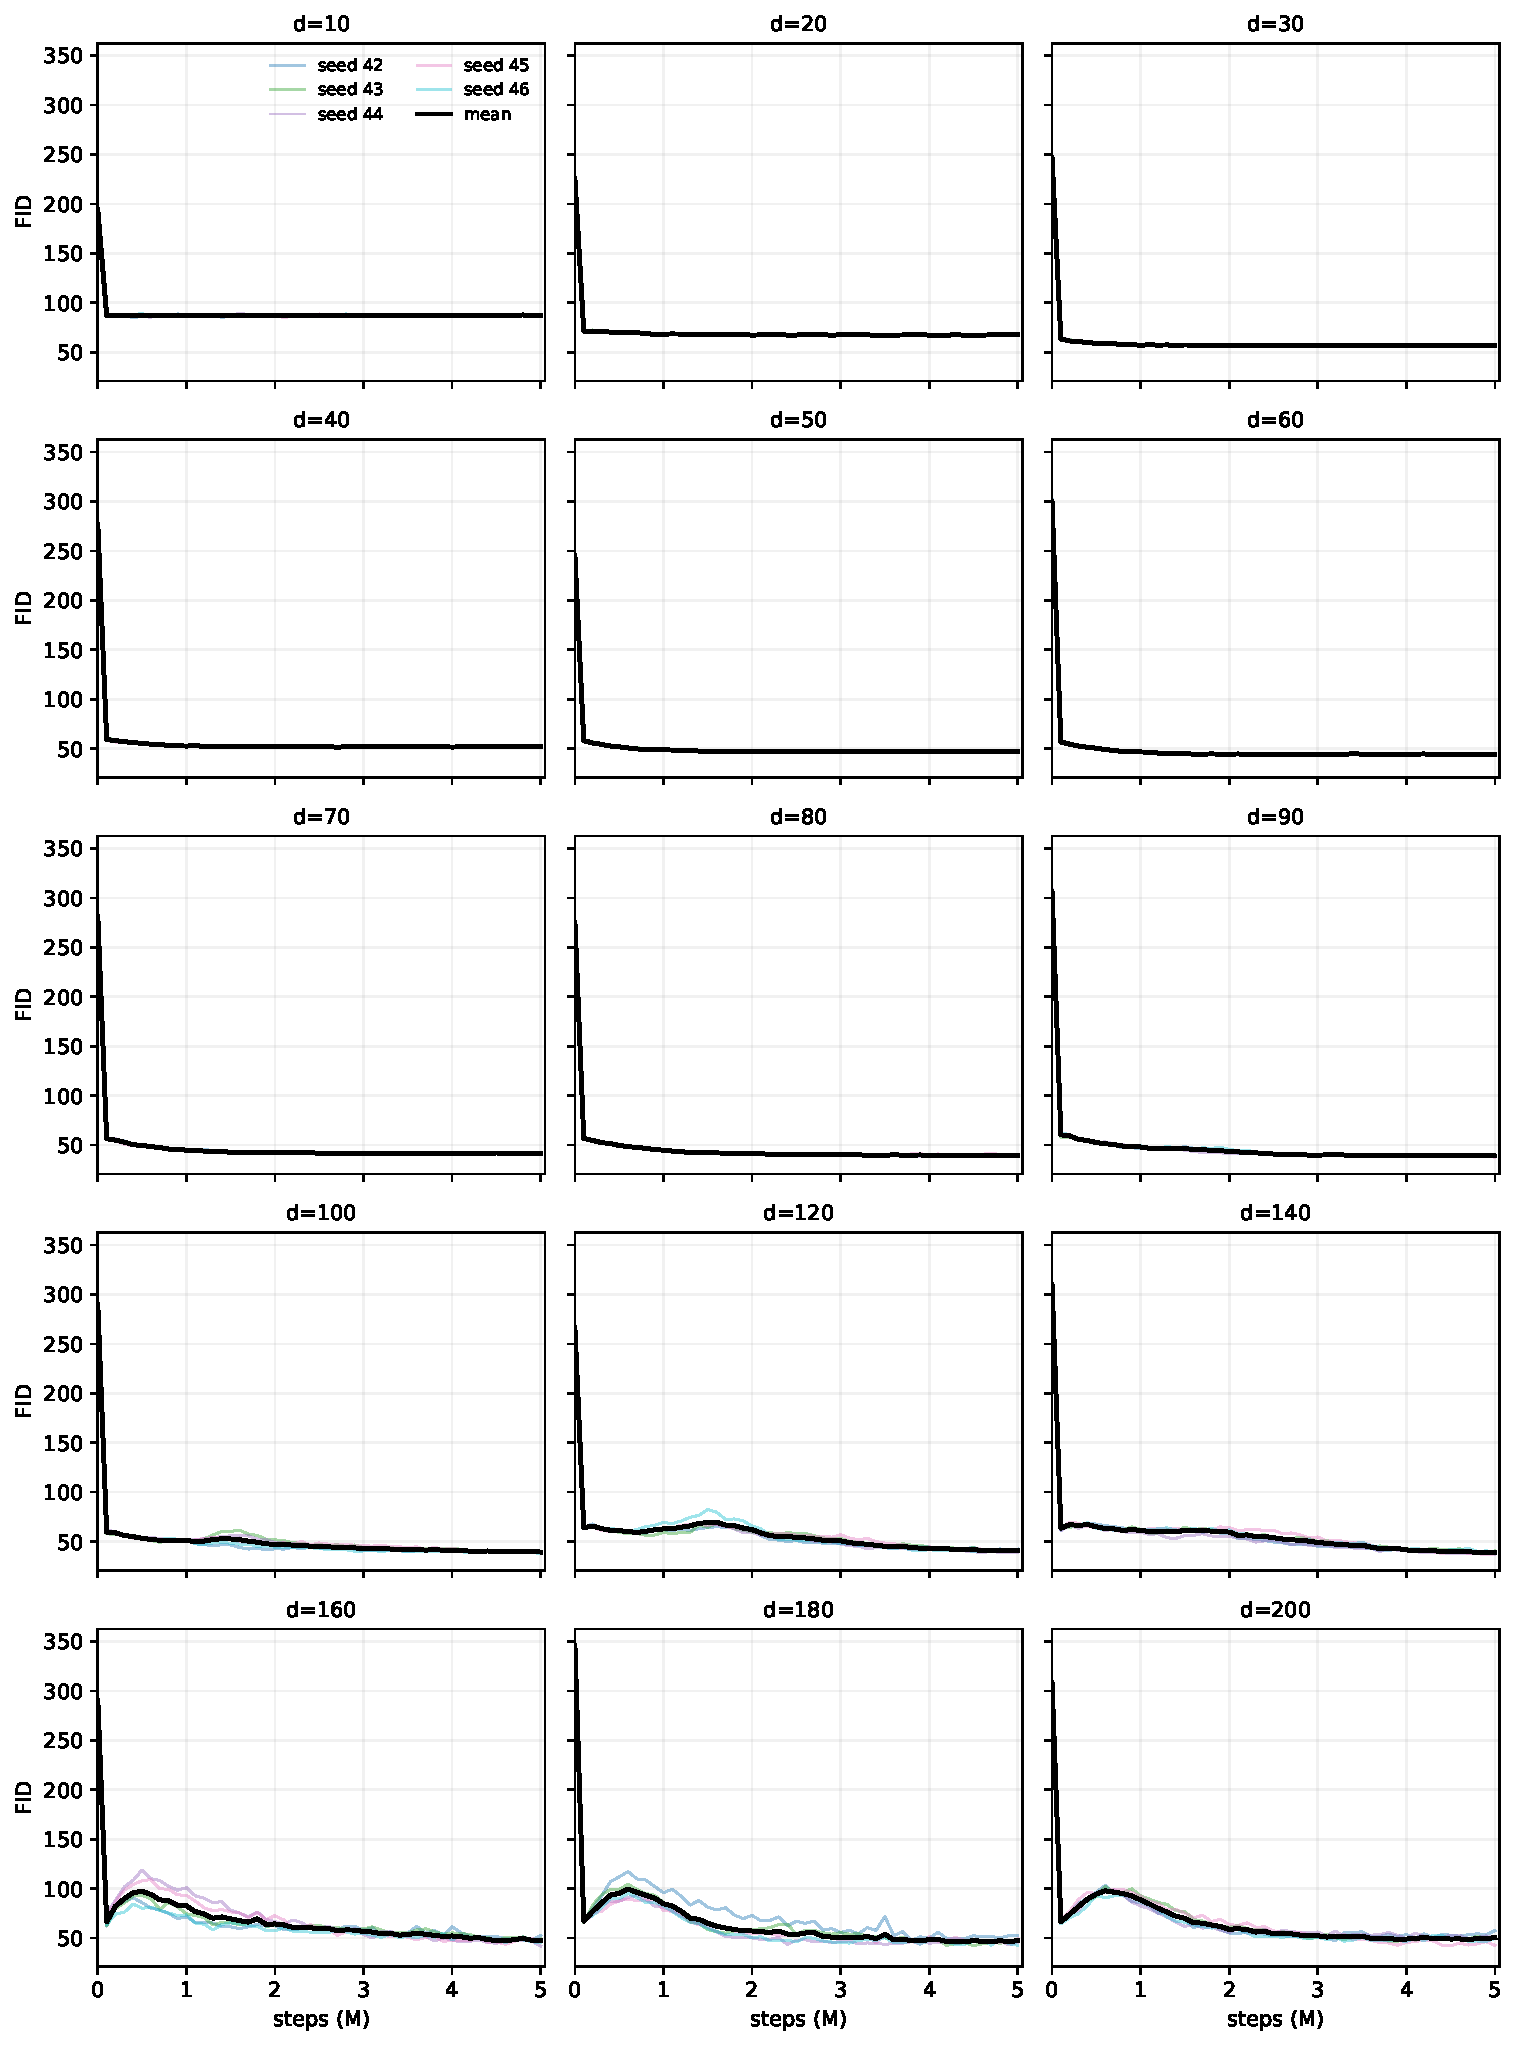
\includegraphics[width=\linewidth]{figures/celeba_individual_fid_by_d_over_steps.pdf}
    \caption{CelebA FID.}
  \end{subfigure}\hfill
  \begin{subfigure}{0.49\linewidth}
    \centering
    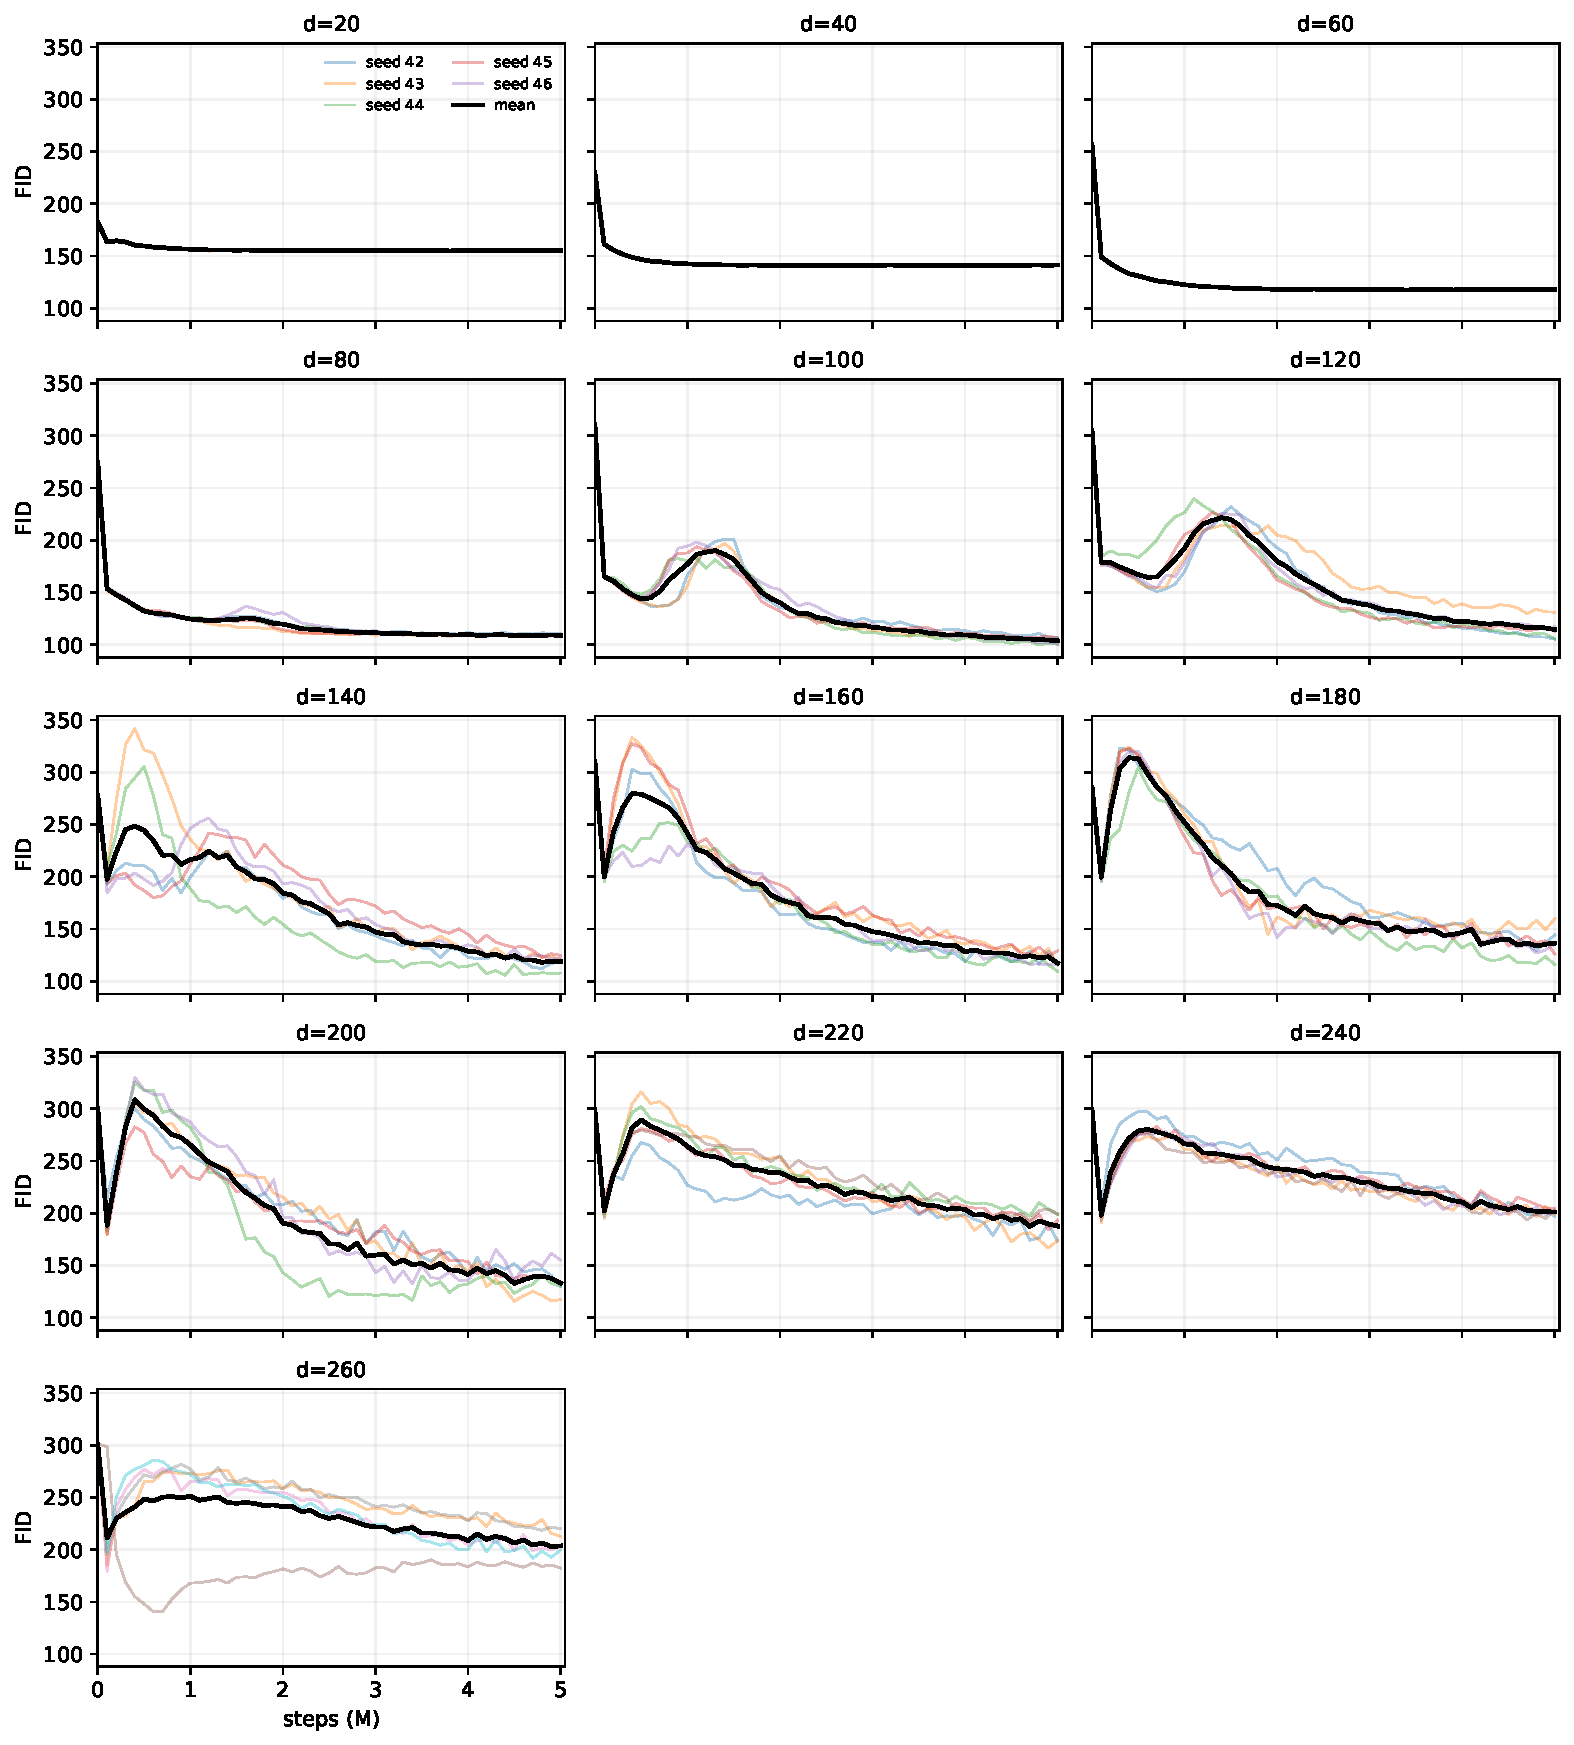
\includegraphics[width=\linewidth]{figures/cifar10_individual_fid_by_d_over_steps.pdf}
    \caption{CIFAR-10 FID.}
  \end{subfigure}
  \caption{\textbf{Per-$\dlat$ FID trajectories.} These are the
    per-dimension panels underlying the aggregate FID curves in the
    body.}
  \label{fig:real-per-d-fid}
\end{figure}

\subsection{Additional spectral predictor diagnostics}

\begin{figure}[!t]
  \centering
  \begin{subfigure}{0.49\linewidth}
    \centering
    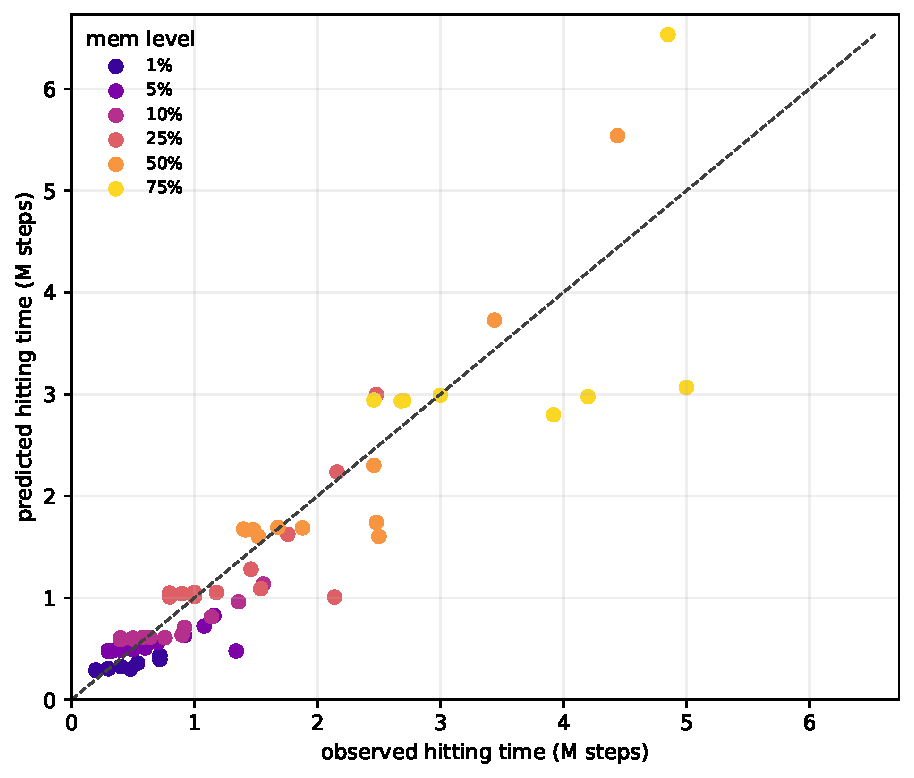
\includegraphics[width=\linewidth]{figures/celeba_spectral_tau_pred_vs_obs.pdf}
    \caption{CelebA.}
  \end{subfigure}\hfill
  \begin{subfigure}{0.49\linewidth}
    \centering
    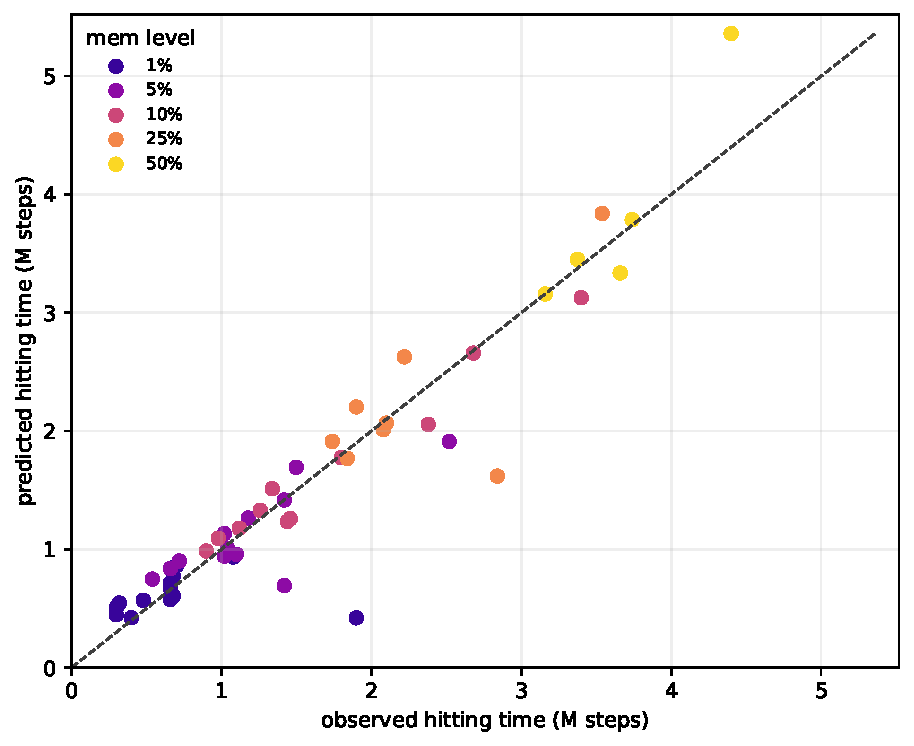
\includegraphics[width=\linewidth]{figures/cifar10_spectral_tau_pred_vs_obs.pdf}
    \caption{CIFAR-10.}
  \end{subfigure}
  \caption{\textbf{Predicted versus observed hitting times.} Each
    point is an iso-memorization threshold for a latent dimension.
    The predictor is calibrated globally across dimensions within a
    dataset.}
  \label{fig:spectral-pred-vs-obs}
\end{figure}

\begin{figure}[!t]
  \centering
  \begin{subfigure}{0.49\linewidth}
    \centering
    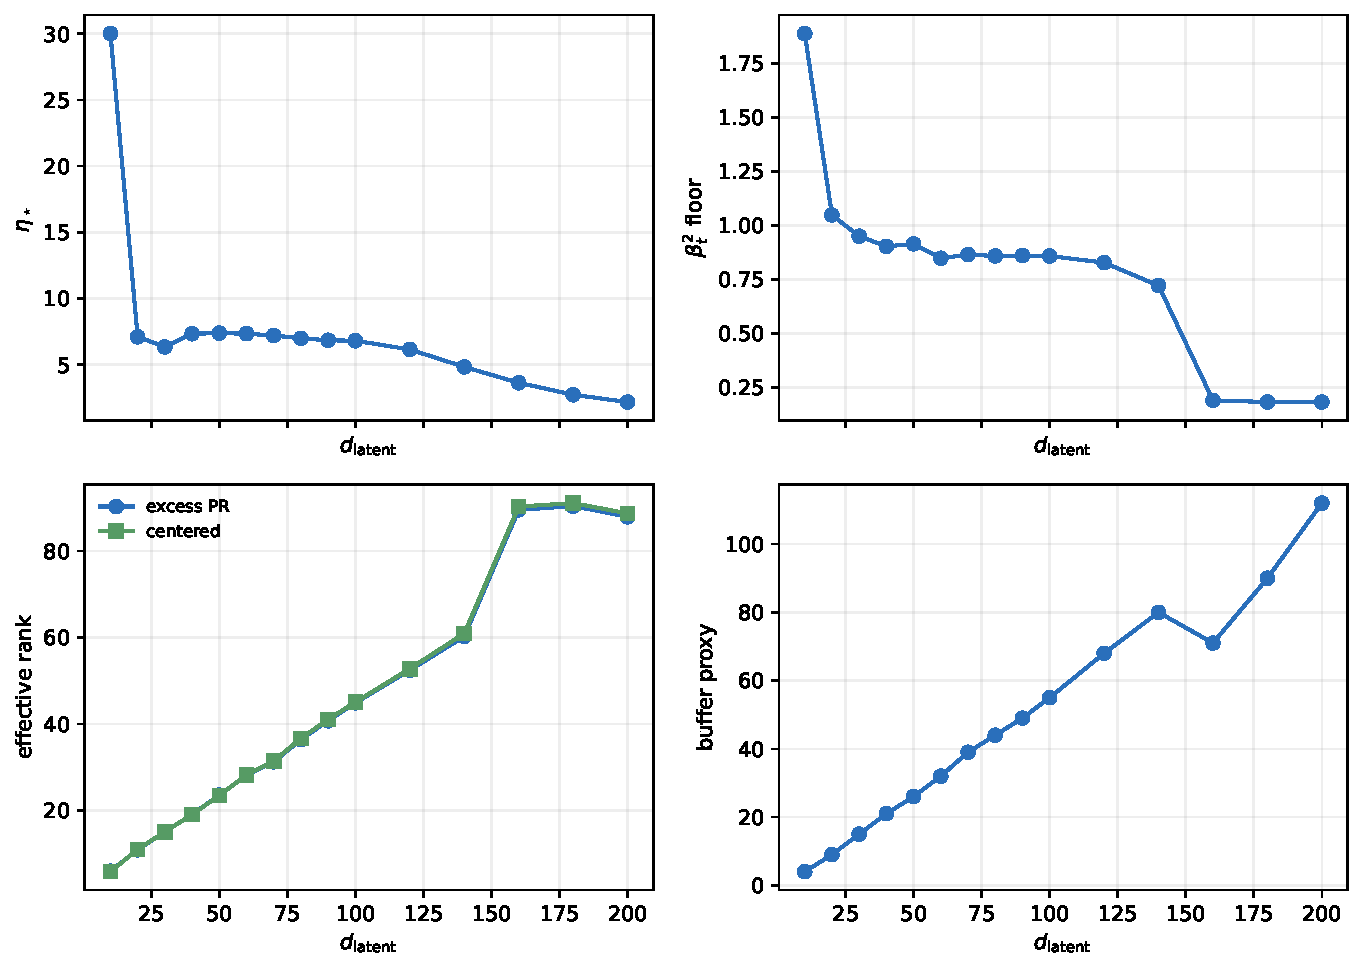
\includegraphics[width=\linewidth]{figures/celeba_spectral_features_vs_d.pdf}
    \caption{CelebA.}
  \end{subfigure}\hfill
  \begin{subfigure}{0.49\linewidth}
    \centering
    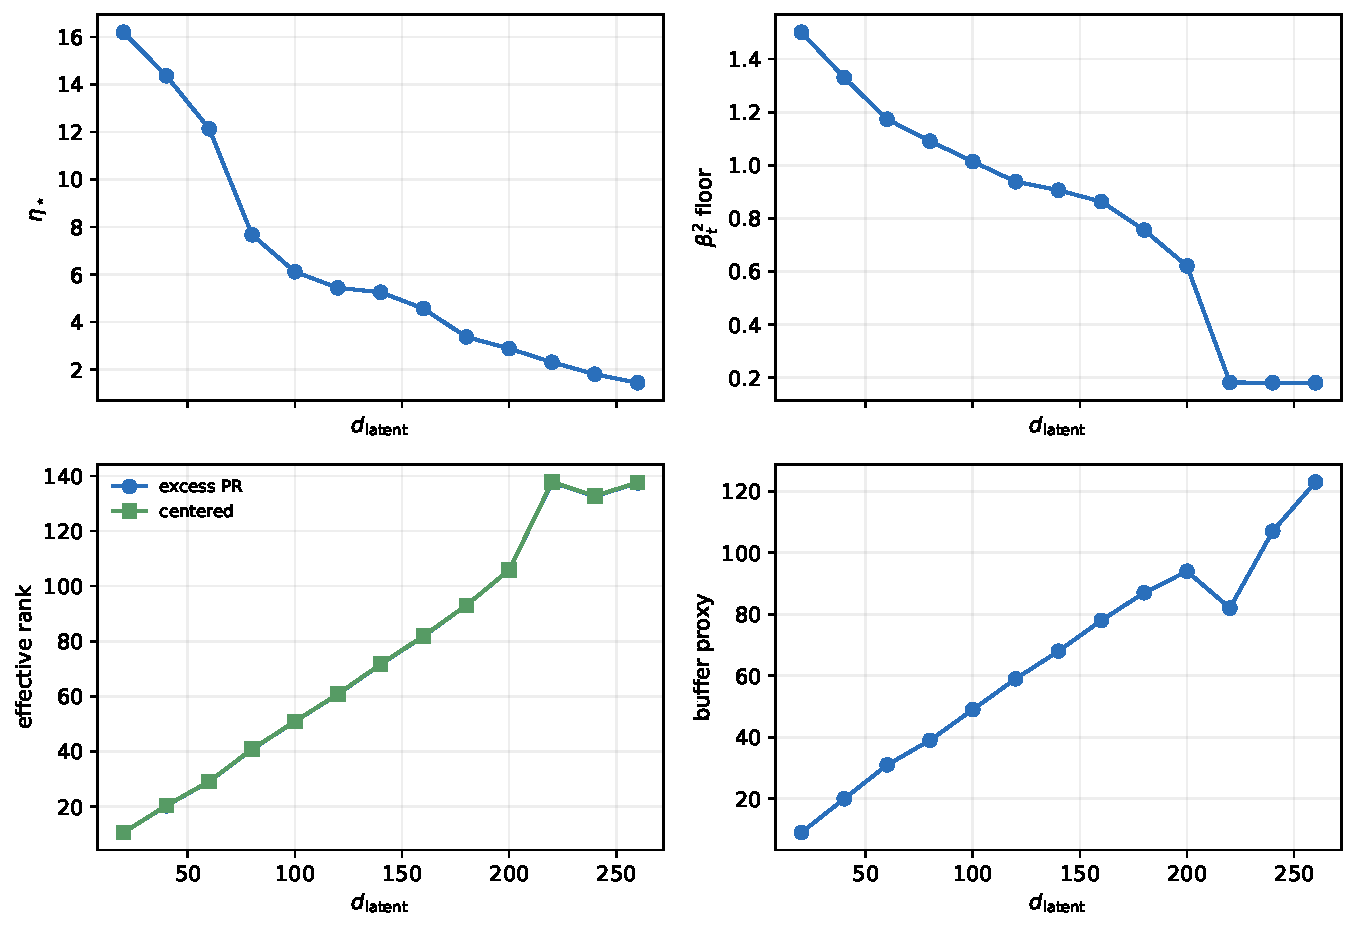
\includegraphics[width=\linewidth]{figures/cifar10_spectral_features_vs_d.pdf}
    \caption{CIFAR-10.}
  \end{subfigure}
  \caption{\textbf{Latent spectral features.} Eigenvalue summaries,
    effective rank, residual-mass proxy, and buffer proxy used by
    the data-spectrum surrogate.}
  \label{fig:spectral-features}
\end{figure}

% ===== RFNN block (sec 4 in the body) ==========================

\section{RFNN: structural justification of the setup}
\label{app:rfnn-justification}

The RFNN of Eq.~\eqref{eq:rfnn} is a deliberately constrained model
and three of its design choices warrant explanation.

\paragraph{Why freeze the first layer.}
Freezing $W$ makes the score-matching loss quadratic in the trained
readout $A$, so gradient flow on $A$ is the linear ODE
Eq.~\eqref{eq:rfnn-gradflow} and admits the closed-form spectral
decomposition that underlies every claim in Section~\ref{sec:rfnn}.
A trainable first layer would couple all weights nonlinearly and
require either a feature-learning theory \citep{mei2018meanfield} or
a lazy / NTK regime \citep{jacot2018ntk}; neither delivers the
explicit per-mode timescale $\tau_i = 1/\lambda_i$ we use to label
$\taugen$ and $\taumem$. \citet{bonnaire2025} establish that the
frozen-feature RFNN reproduces the qualitative two-bulk
generalization/memorization picture observed in trainable networks,
so we adopt their setup directly and inherit its tractability.

\paragraph{Why fix $t = 0.01$.}
Score matching at a single small diffusion time is the regime in
which the population score is sharpest and memorization is most
acute (the noise-to-signal ratio is smallest). Training at one
fixed $t$ removes the time-integration in standard score matching
without changing the spectral structure of $\Umat$, since
$\phi(x_t)$ depends on $t$ only through the diffused state's
covariance. This matches \citeauthor{bonnaire2025}'s setup and
isolates the spectral mechanism from time-averaging effects.

\paragraph{Why $\tanh$ and $\psi_p = \pwidth / \dlat = 64$.}
$\tanh$ is the activation \citet{bonnaire2025} analyze and the
saturation pitfall (Appendix~\ref{app:saturation}) is well
characterized: configurations with $s / \sqrt{\dlat} \lesssim 2$
stay in the regime where the linearised feature map of
Appendix~\ref{app:proof-sketch} applies. The width
$\pwidth = 64\,\dlat$ is chosen to keep the rank-null bulk visible
and the four-bulk structure clearly separated at every $\dlat$;
smaller $\pwidth$ collapses the rank-null and sample bulks because
$\pwidth - \dlat - \nsamp$ shrinks, while much larger $\pwidth$
provides no additional structural information at fixed
$\nsamp / \dlat$.

\paragraph{Connection to the trainable MLP.}
The Section~\ref{sec:mlp} MLP results recover the same buffer
mechanism qualitatively (delayed $\taumem$, monotone late
gen-gap), confirming that the RFNN idealization is not a degenerate
case of the broader feature-learning picture but a tractable
representative of it.

\section{RFNN: sketch of an analytical derivation}
\label{app:proof-sketch}

We sketch the extension of \citeauthor{bonnaire2025}'s replica
computation to block-diagonal data covariance
$\Sigmadata = \diag\!\bigl(\sigsig^2\mathbb{I}_{\dint},\,
\signoise^2\mathbb{I}_{\dlat - \dint}\bigr)$. Throughout,
$x^\mu = m_{c(\mu)} + \xi^\mu$ with $m_{c(\mu)}$ a cluster center in
the $\dint$-dimensional signal subspace and $\xi^\mu \sim
\mathcal{N}(0, \Sigmadata)$. The diffused state at time $t$ is
$x_t^\mu = e^{-t}\,x^\mu + \sqrt{\Delta_t}\,\eta^\mu$ with
$\Delta_t = 1 - e^{-2t}$ and $\eta^\mu \sim \mathcal{N}(0, \mathbb{I}_{\dlat})$.

\paragraph{Linearised feature map.}
For data scale $s$ small compared with $\sqrt{\dlat}$ (the regime in
which our experiments operate; cf.~Appendix~\ref{app:saturation}),
$\tanh(Wx/\sqrt{\dlat}) \approx Wx/\sqrt{\dlat} - \tfrac{1}{3}(Wx)^3/\dlat^{3/2}$,
and to leading order $\phi(x) = (1/\sqrt{\pwidth})\tanh(Wx/\sqrt{\dlat})
\approx Wx/\sqrt{\pwidth\dlat}$. The linearised correlation matrix is
\begin{equation}
  \Umat^{\mathrm{lin}} = \tfrac{1}{\pwidth\dlat}\,W\,M_t\,W^\top,
  \qquad
  M_t \;:=\; \tfrac{1}{\nsamp}\sum_{\mu} \E_{\eta}\!\bigl[x_t^\mu (x_t^\mu)^\top\bigr],
  \label{eq:U-lin}
\end{equation}
which factors $\Umat$'s spectrum into the spectra of $W^\top W$ and
$M_t$, the latter inheriting the block-diagonal geometry of
$\Sigmadata$.

\paragraph{Block decomposition of $M_t$.}
Direct computation gives
\begin{equation}
  M_t \;=\; e^{-2t}\bigl(\hat C + \hat S\bigr) + \Delta_t\,\mathbb{I}_{\dlat},
  \label{eq:Mt}
\end{equation}
where $\hat C = \tfrac{1}{\nsamp}\sum_\mu m_{c(\mu)}m_{c(\mu)}^\top$
is the empirical centroid Gram matrix and $\hat S =
\tfrac{1}{\nsamp}\sum_\mu \xi^\mu(\xi^\mu)^\top$ is the empirical
within-cluster covariance. In population,
$\E\hat C = (1/k)\sum_c m_c m_c^\top$ has rank $\dint$ with eigenvalues
$\Theta(s^2/\dint)$ in the signal subspace; $\E\hat S = \Sigmadata$
has eigenvalues $\sigsig^2$ on the signal block and $\signoise^2$ on
the null block. The sample fluctuations $\hat S - \Sigmadata$ are
rank-$\nsamp$ with spectrum given by a Marchenko-Pastur-type law
\citep{ELKaroui2010spectrum, couillet2011rmt} of typical scale
$\Sigmadata/\sqrt{\nsamp}$ in operator norm.

\paragraph{Four bulks from rank addition.}
$M_t$ thus splits into three rank classes:
\begin{enumerate}\itemsep1pt
  \item[\textbf{(a)}] \emph{Population signal} ($\dint$ modes):
        eigenvalues $e^{-2t}\bigl[s^2/\dint + \sigsig^2\bigr] +
        \Delta_t$, dominated by the cluster scale.
  \item[\textbf{(b)}] \emph{Population null} ($\dlat - \dint$ modes):
        eigenvalues $e^{-2t}\signoise^2 + \Delta_t$, set by either
        the null-space data variance or the diffusion noise floor,
        whichever is larger.
  \item[\textbf{(c)}] \emph{Sample fluctuation} ($\nsamp$ modes):
        eigenvalues of $e^{-2t}(\hat S - \Sigmadata)$ projected onto
        the signal subspace, scaling as
        $\Theta\!\bigl(e^{-2t}\sigsig^2/\sqrt{\nsamp}\bigr)$, plus a
        smaller contribution in the null subspace.
\end{enumerate}
Lifting through $W$ via Eq.~\eqref{eq:U-lin} and noting that
$W^\top W / \dlat$ has bulk spectrum on $[(\sqrt{\pwidth/\dlat} -
1)^2,\,(\sqrt{\pwidth/\dlat} + 1)^2]$ for $\pwidth \gg \dlat$
\citep{pennington2017nonlinear}, $\Umat^{\mathrm{lin}}$ inherits the
three rank classes from $M_t$ plus a fourth, trivial \emph{rank-null}
class of size $\pwidth - \dlat - \nsamp$ from the null space of the
sample-fluctuation projector, accounting for all four bulks reported
in Section~\ref{sec:rfnn}.

\paragraph{Bulk-gap scaling.}
The signal-to-null gap is
$\Theta\!\bigl(s^2/(\dint\signoise^2)\bigr)$ (when
$\signoise^2 \gtrsim \Delta_t$) or $\Theta\!\bigl(s^2/(\dint\Delta_t)\bigr)$
(when $\signoise^2 \lesssim \Delta_t$); the null-to-sample gap is
$\Theta\!\bigl(\sqrt{\nsamp}\,\signoise^2/\sigsig^2\bigr)$ when the
null block dominates the diffusion noise, shrinking smoothly to
$O(1)$ as $\signoise^2 \to \Delta_t$. The four-bulk picture is
observable whenever $\sigsig^2 \gg \max(\signoise^2, \Delta_t) \gg
1/\sqrt{\nsamp}$. A fully rigorous derivation requires a Stieltjes
transform calculation along the lines of
\citet{bonnaire2025, ELKaroui2010spectrum, benigni2021eigenvalue}
extended to block-diagonal $\Sigmadata$, plus a control of the
nonlinear $\tanh$ corrections beyond the leading linear term. We
leave this to follow-up work.

\section{RFNN: eigenvalue saturation and the $\tanh$ pitfall}
\label{app:saturation}

We observed that for sufficiently large data scale $s$, the spectrum of
$\Umat$ collapses to a single bulk with eigenvalues bunched at
$\lambda \approx 1$. The cause is $\tanh$ saturation: when
$\|Wx\|/\sqrt{\dlat} \gtrsim 2$, $\tanh$ outputs $\pm 1$ almost
deterministically and the feature map becomes effectively constant in
$x$. The constraint $s/\sqrt{\dlat} \lesssim 2$ defines the safe
operating regime; all reported sweeps satisfy this constraint.

\section{RFNN: empirical bulk detection}
\label{app:bulk-detection}

Fig.~\ref{fig:bulk-sizes-distances} shows the $\signoise = 0.01$
$\dlat$ sweep with the empirical bulk-detection overlay (peaks
found by \texttt{scipy.signal.find\_peaks} on the histogram counts,
capped at 4 by prominence). At the larger anisotropy ratio
$\sigsig^2/\signoise^2 \approx 10^4$ the four bulks separate
cleanly and the detected peaks land where the theoretical
index-based cuts in Fig.~\ref{fig:fourbulk-hist} put them.

\begin{figure}[!t]
  \centering
  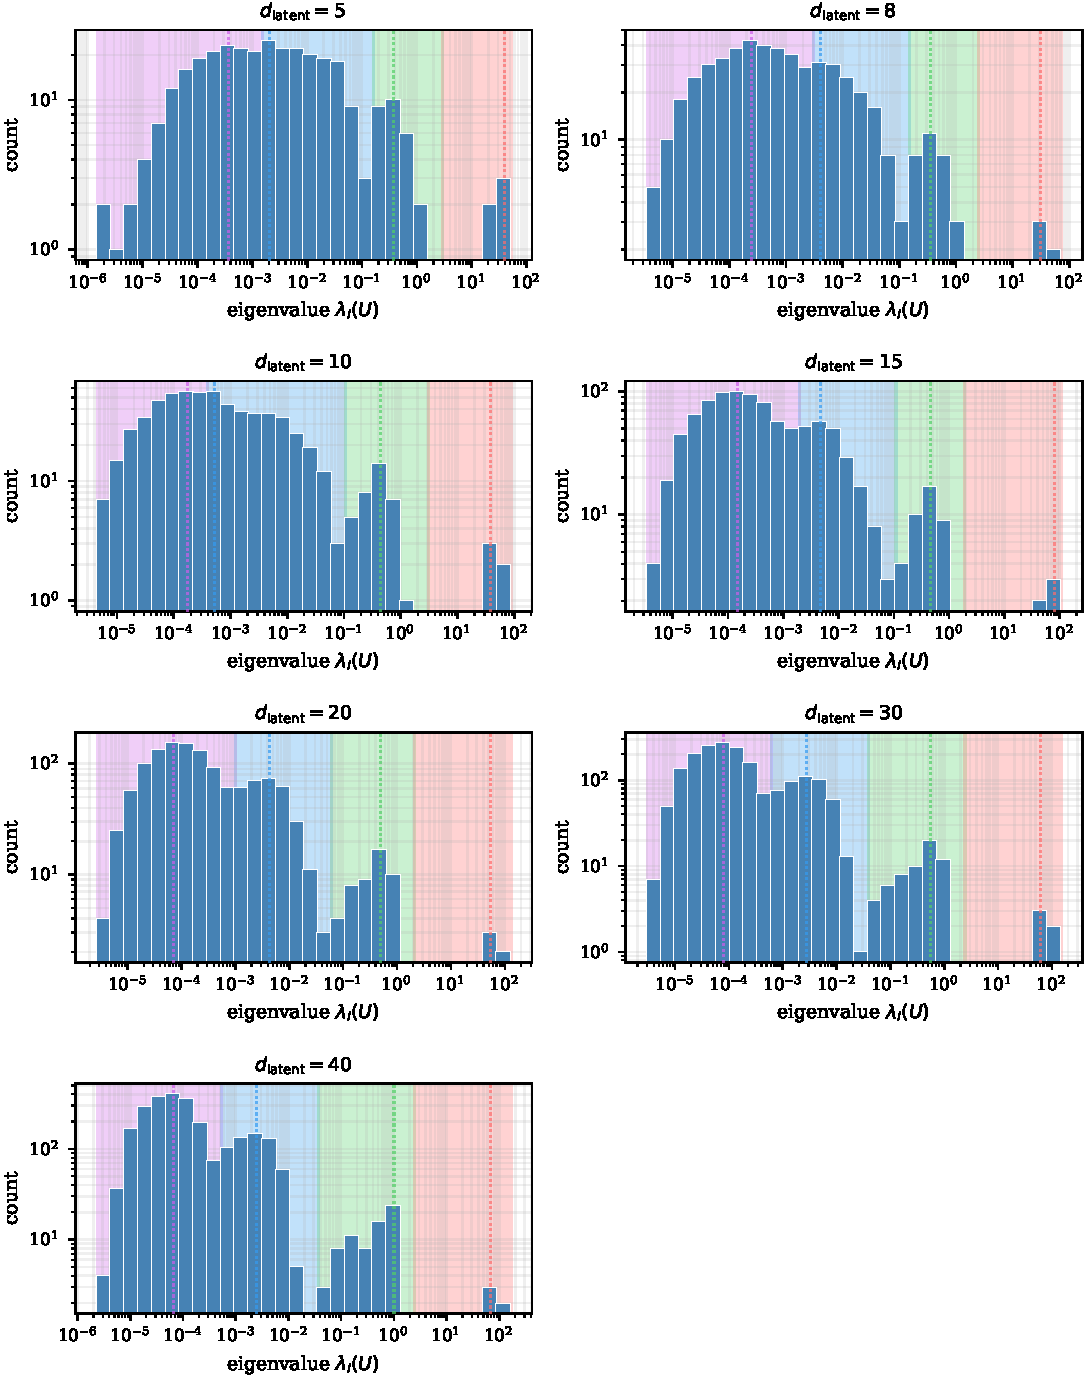
\includegraphics[width=\linewidth]{figures/bulk_detection_hist.pdf}
  \caption{\textbf{Empirical bulk detection across the $\dlat$
    sweep at $\signoise = 0.01$.} Each colored region is one
    detected peak in the eigenvalue density; four bulks are
    detected in every panel. As $\dlat / \dint$ grows, the bulks
    pull apart: at $\dlat = \dint$ the four peaks sit close
    together with shallow valleys, and by $\dlat = 40$
    ($\dlat / \dint = 8$) they have separated into well-isolated
    peaks decades apart in eigenvalue. Per-panel bulk sizes are
    tabulated in Table~\ref{tab:bulk-sizes}; detection algorithm
    in Appendix~\ref{app:methods}.}
  \label{fig:bulk-sizes-distances}
\end{figure}

\section{RFNN: additional 4-bulk spectrum figures}
\label{app:appendix-figures}

The body shows the $\signoise = 0.5$ density view
(Figure~\ref{fig:fourbulk-hist}); for completeness we include the
remaining three corners of the $\{\text{cliffs}, \text{density}\}
\times \{\signoise = 0.01, 0.5\}$ grid here.
Figures~\ref{fig:appendix-fourbulk-cliffs}
and~\ref{fig:appendix-fourbulk-cliffs-sn05} are the cliffs (sorted-spectrum)
view at the two noise scales, and
Figure~\ref{fig:appendix-fourbulk-hist-sn001} is the density view
at $\signoise = 0.01$.
Figure~\ref{fig:appendix-fourbulk-dint} sweeps $\dint$ instead of $\dlat$.

\begin{figure}[!t]
  \centering
  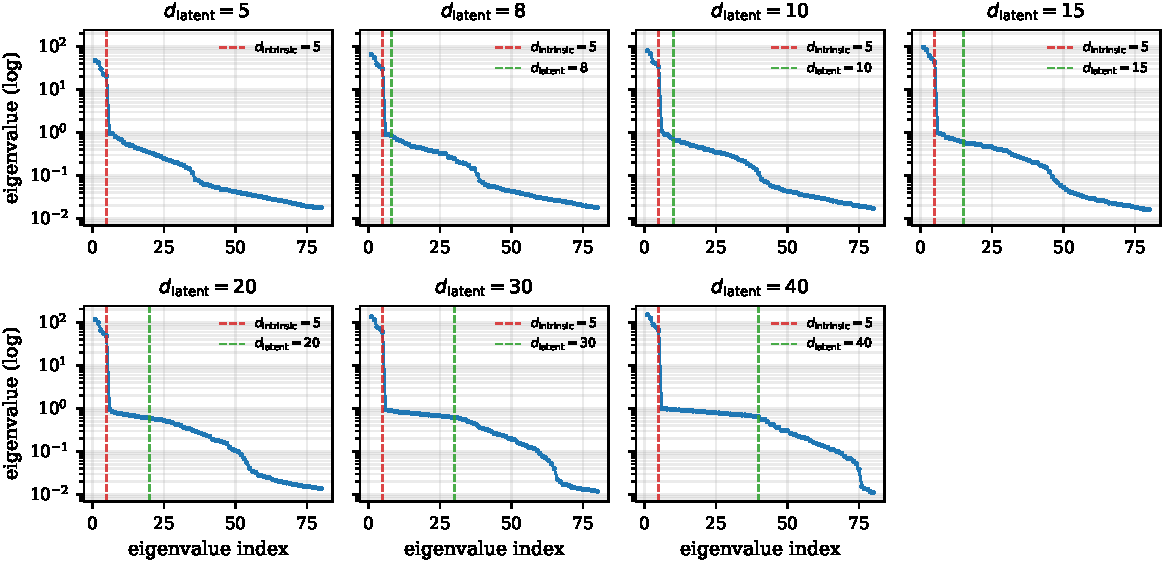
\includegraphics[width=\linewidth]{figures/four_bulk_dlat_sweep.pdf}
  \caption{\textbf{Cliffs view, $\signoise = 0.01$.}
    Sorted log-spectrum across the $\dlat$ sweep. Red and green
    dashed lines mark indices $\dint$ and $\dlat$. The
    $\textsc{bulk\_data\_noise}$ region widens between them as
    $\dlat$ grows.}
  \label{fig:appendix-fourbulk-cliffs}
\end{figure}

\begin{figure}[!t]
  \centering
  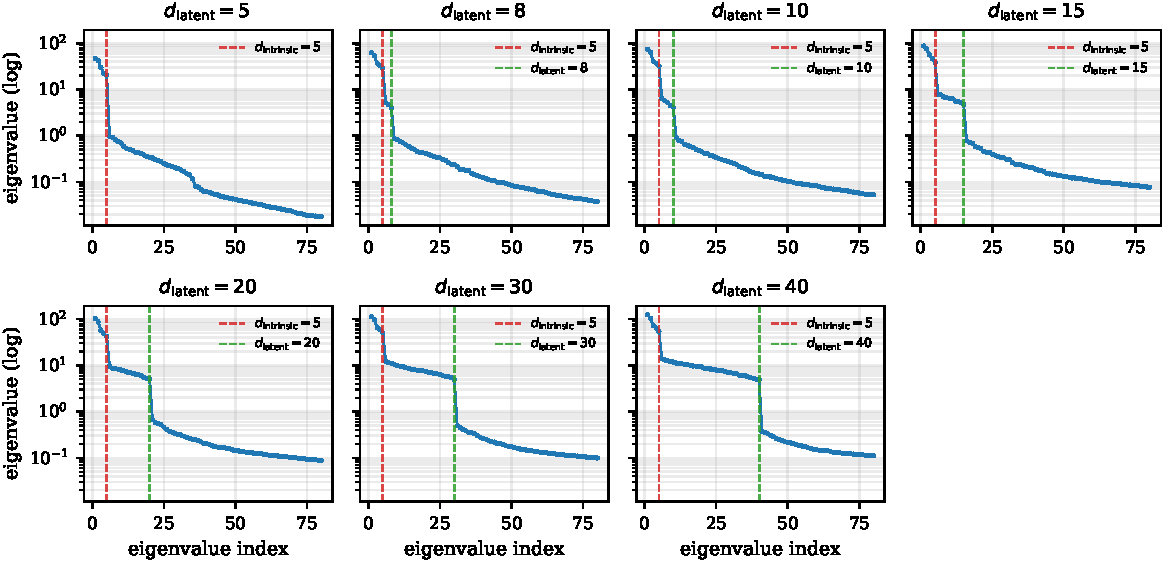
\includegraphics[width=\linewidth]{figures/four_bulk_dlat_sweep_sn05.pdf}
  \caption{\textbf{Cliffs view, $\signoise = 0.5$.}
    Same sweep as Figure~\ref{fig:appendix-fourbulk-cliffs} at the
    higher noise scale: the signal/noise-dim cliff at index $\dint$
    is sharp, while the data/sample cliff at index $\dlat$ softens
    as the gap $\sigsig^2/\signoise^2$ shrinks.}
  \label{fig:appendix-fourbulk-cliffs-sn05}
\end{figure}

\begin{figure}[!t]
  \centering
  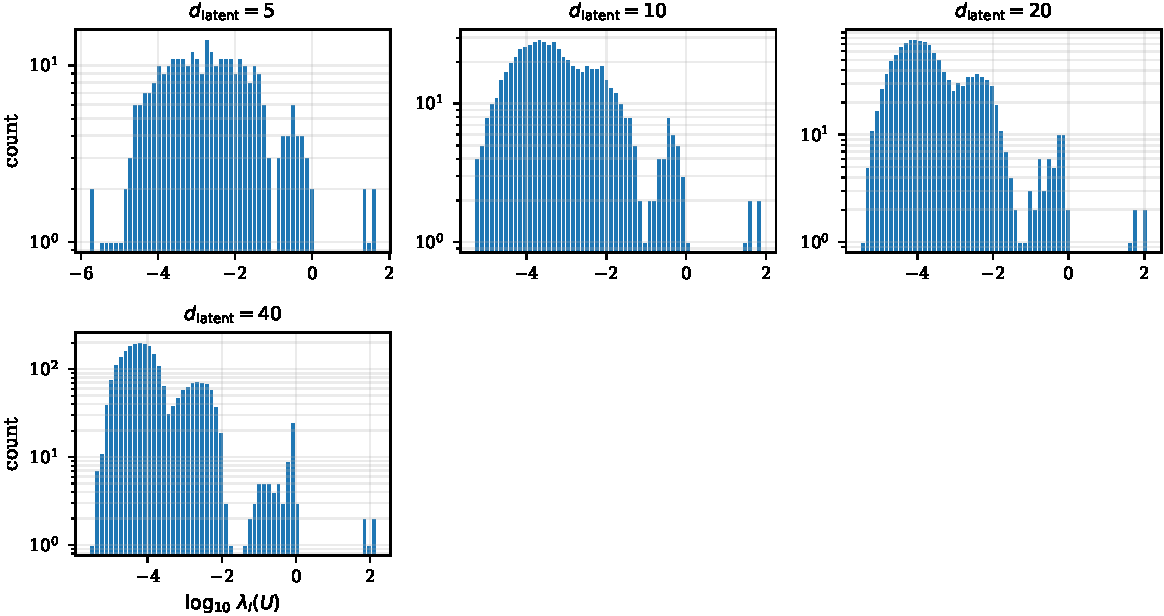
\includegraphics[width=\linewidth]{figures/four_bulk_dlat_hist_sn001.pdf}
  \caption{\textbf{Density view, $\signoise = 0.01$.}
    Counterpart to the body's Figure~\ref{fig:fourbulk-hist}. The
    larger $\sigsig^2/\signoise^2 \approx 10^4$ pushes the signal
    bulk decades to the right of the noise-dim bulk.}
  \label{fig:appendix-fourbulk-hist-sn001}
\end{figure}

\begin{figure}[!t]
  \centering
  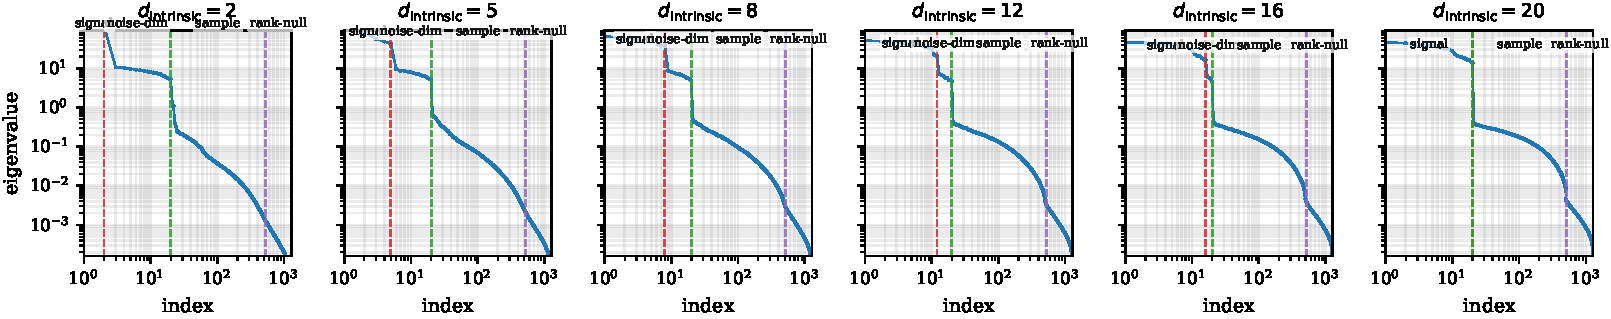
\includegraphics[width=\linewidth]{figures/four_bulk_dint_sweep.pdf}
  \caption{\textbf{Varying $\dint$} at $\dlat = 20$,
    $\signoise = 0.5$. As $\dint \to \dlat$ the noise-dim bulk
    shrinks toward zero width and we recover Bonnaire's two-bulk
    picture.}
  \label{fig:appendix-fourbulk-dint}
\end{figure}
